\section{State of the Art}\label{chap:standdertechnik}
\subsection{The Fundamentals of Light}
Light is a substantial part of the universe. It lets us see the world, the stars and has remarkable properties in the space-time. For example it is the fastest way of energy transportation with a speed of $c = 299792458~m/s$ in vacuum. The definition of electromagnetic radiation gathers all kinds of light like visible (VIS), infrared (IR), ultraviolet light (UV) and other kinds of radiation like microwaves or radio waves. James Clerk Maxwell discovered that light can be described by an electric $\vec{E}$ and a magnetic $\vec{M}$ field that stand perpendicular to each other and to the direction of wave propagation. Figure \ref{fig:LightasWave} shows the propagation of one light ray. Both fields oscillated with the same wavelength of the light $\lambda$ and the frequency $\nu$ moving into the wave direction of the wave vector propagation. Green light for example is defined within 520 and 565 nm while radio waves have a length of several meters. With shorter wavelength, the energy of the photon increases and interaction with material changes. Figure \ref{fig:EM_spectrum} shows the complete electromagnetic spectrum from $\gamma$-rays to long radio waves. With shorter wavelengths, the radiation causes interactions at the atomic and subatomic level.
\begin{figure}[!h]
	\centering  
	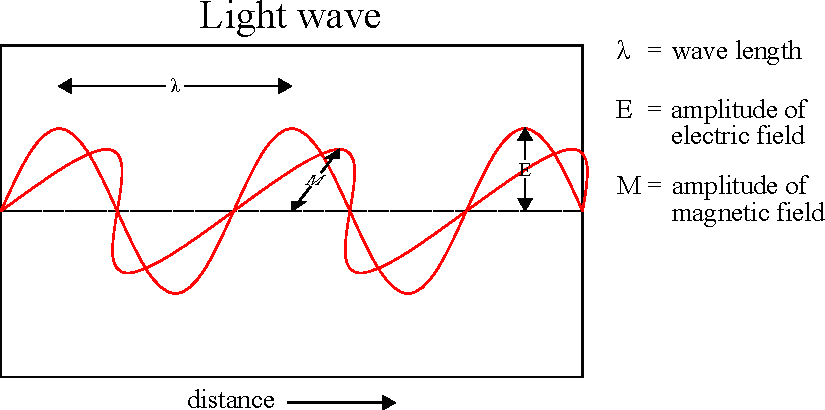
\includegraphics[width=0.6\linewidth]{Bilder/lightwave.pdf}
	\caption{Light as electromagnetic wave \tiny Gpvos 2007 wikipedia.org \ccbysa }
	\label{fig:LightasWave}
\end{figure}
 
 The polarization of light characterizes how the fields $\vec{E}$ and $\vec{M}$ orientation in space is distributed between different light waves. An unpolarized light source emits a chaotic orientated wave form. After polarized filtering only waves with the same orientation remain. The coherence of light describes correlations in the wavelength and the phase relation between the $\vec{E}$ and $\vec{M}$ oscillation. Coherent light sources cause interference between each other, resulting in a new coherent wave form. The coherence length is the distance of propagation where the wave is still of the same wavelength and phasing and can interfere with itself in the same way. Two interfering coherent waves in the same phase cause constructive interference. The amplitudes will sum up. A phase shift of $180^\circ$ between two coherent waves will result in a destructive interference and a subtraction of amplitudes. Incoherent waves that are polarized can still be monochromatic, meaning that the wave length is in a narrow band in the spectrum. However the phase and directions of the waves are randomly distributed between each other. 

\begin{figure}[!h]
	\centering
	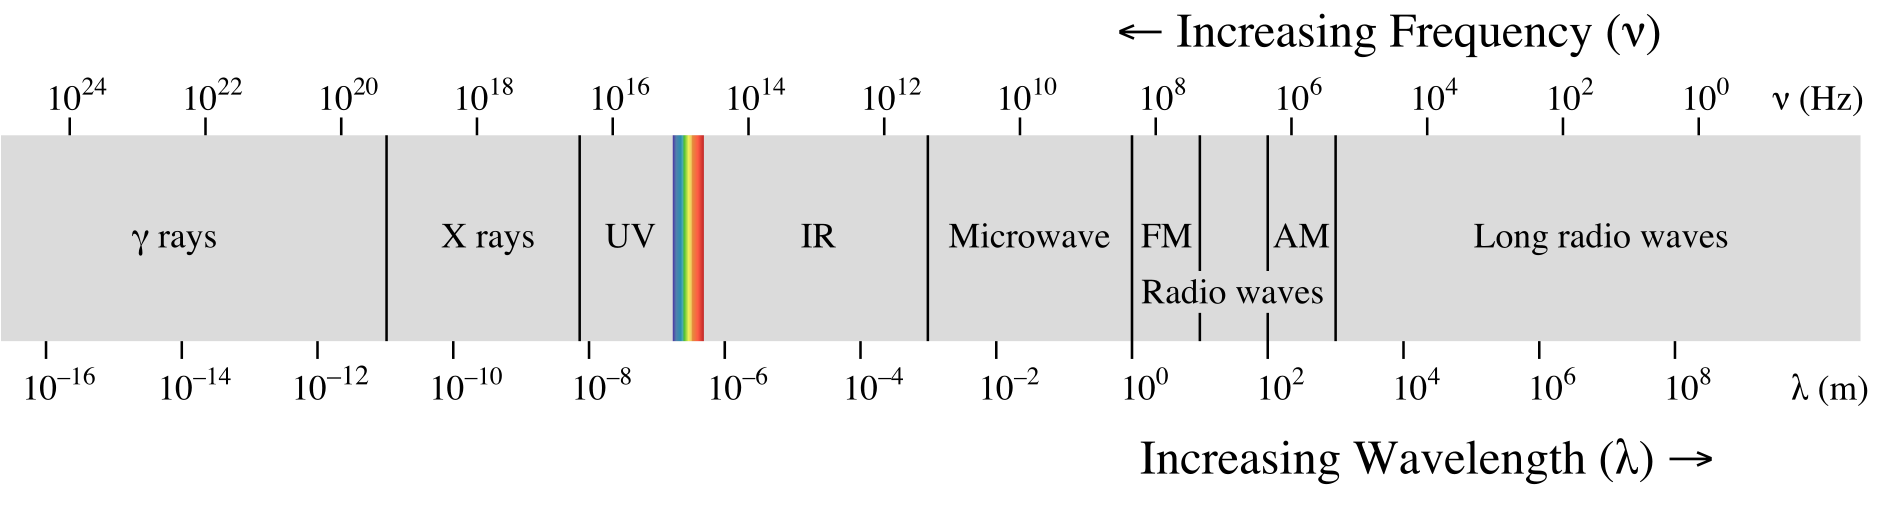
\includegraphics[width=0.7\linewidth]{Bilder/EM_spectrum.png}
	\caption{Electromagnetic spectrum \tiny Philip Ronan wikipedia.org \ccbysa}
	\label{fig:EM_spectrum}
\end{figure}

The Planck constant $h$ specifies the relation between energy E and frequency of light $\nu$. The radiant energy of one light beam can also be considered as a particle with the mass m, a so called photon.

\begin{equation}
 E =  h\cdot \nu=mc^2 ~~ [J]
\end{equation}

\begin{equation}
\lambda = \frac c \nu ~~[m]
\end{equation}
\medskip
 
 The mass-energy equivalence proves that light waves can be transformed into and from mass. This can be observed in the sun. The nuclear fusion of two hydrogen atoms results in a helium atom. A small amount of mass is lost in this reaction and transformed into electromagnetic energy that lightens our universe. The different wavelengths of a light source are represented in the electromagnetic spectrum. The sun's irradiance provides the complete electromagnetic power per square meter that is delivered on a surface in a certain distance. This value is corrected by the wavelengths of the specific light spectrum in the spectral irradiance. Figure \ref{fig:SolarSpectrum} shows the VIS and IR components of the sunlight and how they are influenced by the atmosphere of the earth in the spectral irradiance versus the wavelength.
 
\begin{figure}[!h]
	\centering
	\includegraphics[width=0.5\linewidth]{Bilder/Solar_spectrum.png}
	\caption{Solar radiation spectrum on earth \tiny Nick84 wikipedia.org 2013 \ccbysa}
	\label{fig:SolarSpectrum}
\end{figure}

The atmosphere of the earth absorbs various wavelengths that are related to the gas composition. Water ($H_2O$) and carbon dioxide ($CO_2$) absorb the infrared light of the solar spectrum while ozone ($O_3$) absorbs the high energy UV radiation. Nitrogen ($N_2$), however, is transparent for most components of the sunlight.


\subsection{Photometric and Radiometric Quantities}

Photometric (index v) and radiometric (index e) quantities are used for the quantification of light sources and lighting conditions. The human spectral sensitivity for visible light is considered in the luminosity function. The eye is capable to adapt its spectral sensitivity to different light conditions. Figure \ref{fig:luminosity} shows the CIE standard luminosity function V($\lambda$) in the photopic view under well-lit lighting and the scotopic view under low light. The peak of the photopic sensitivity can be found at about 555 nm which is the base for the normalization of the curve. The CIE luminosity function is a standard established by the Commission International de l'Eclairage and forms the central color matching function for light sources. The radiometric quantities consider the complete electromagnetic spectrum and are independent of the sensitivity of the human eye \cite{mccluney1994introduction}.

\begin{figure}[!h]
	\centering
	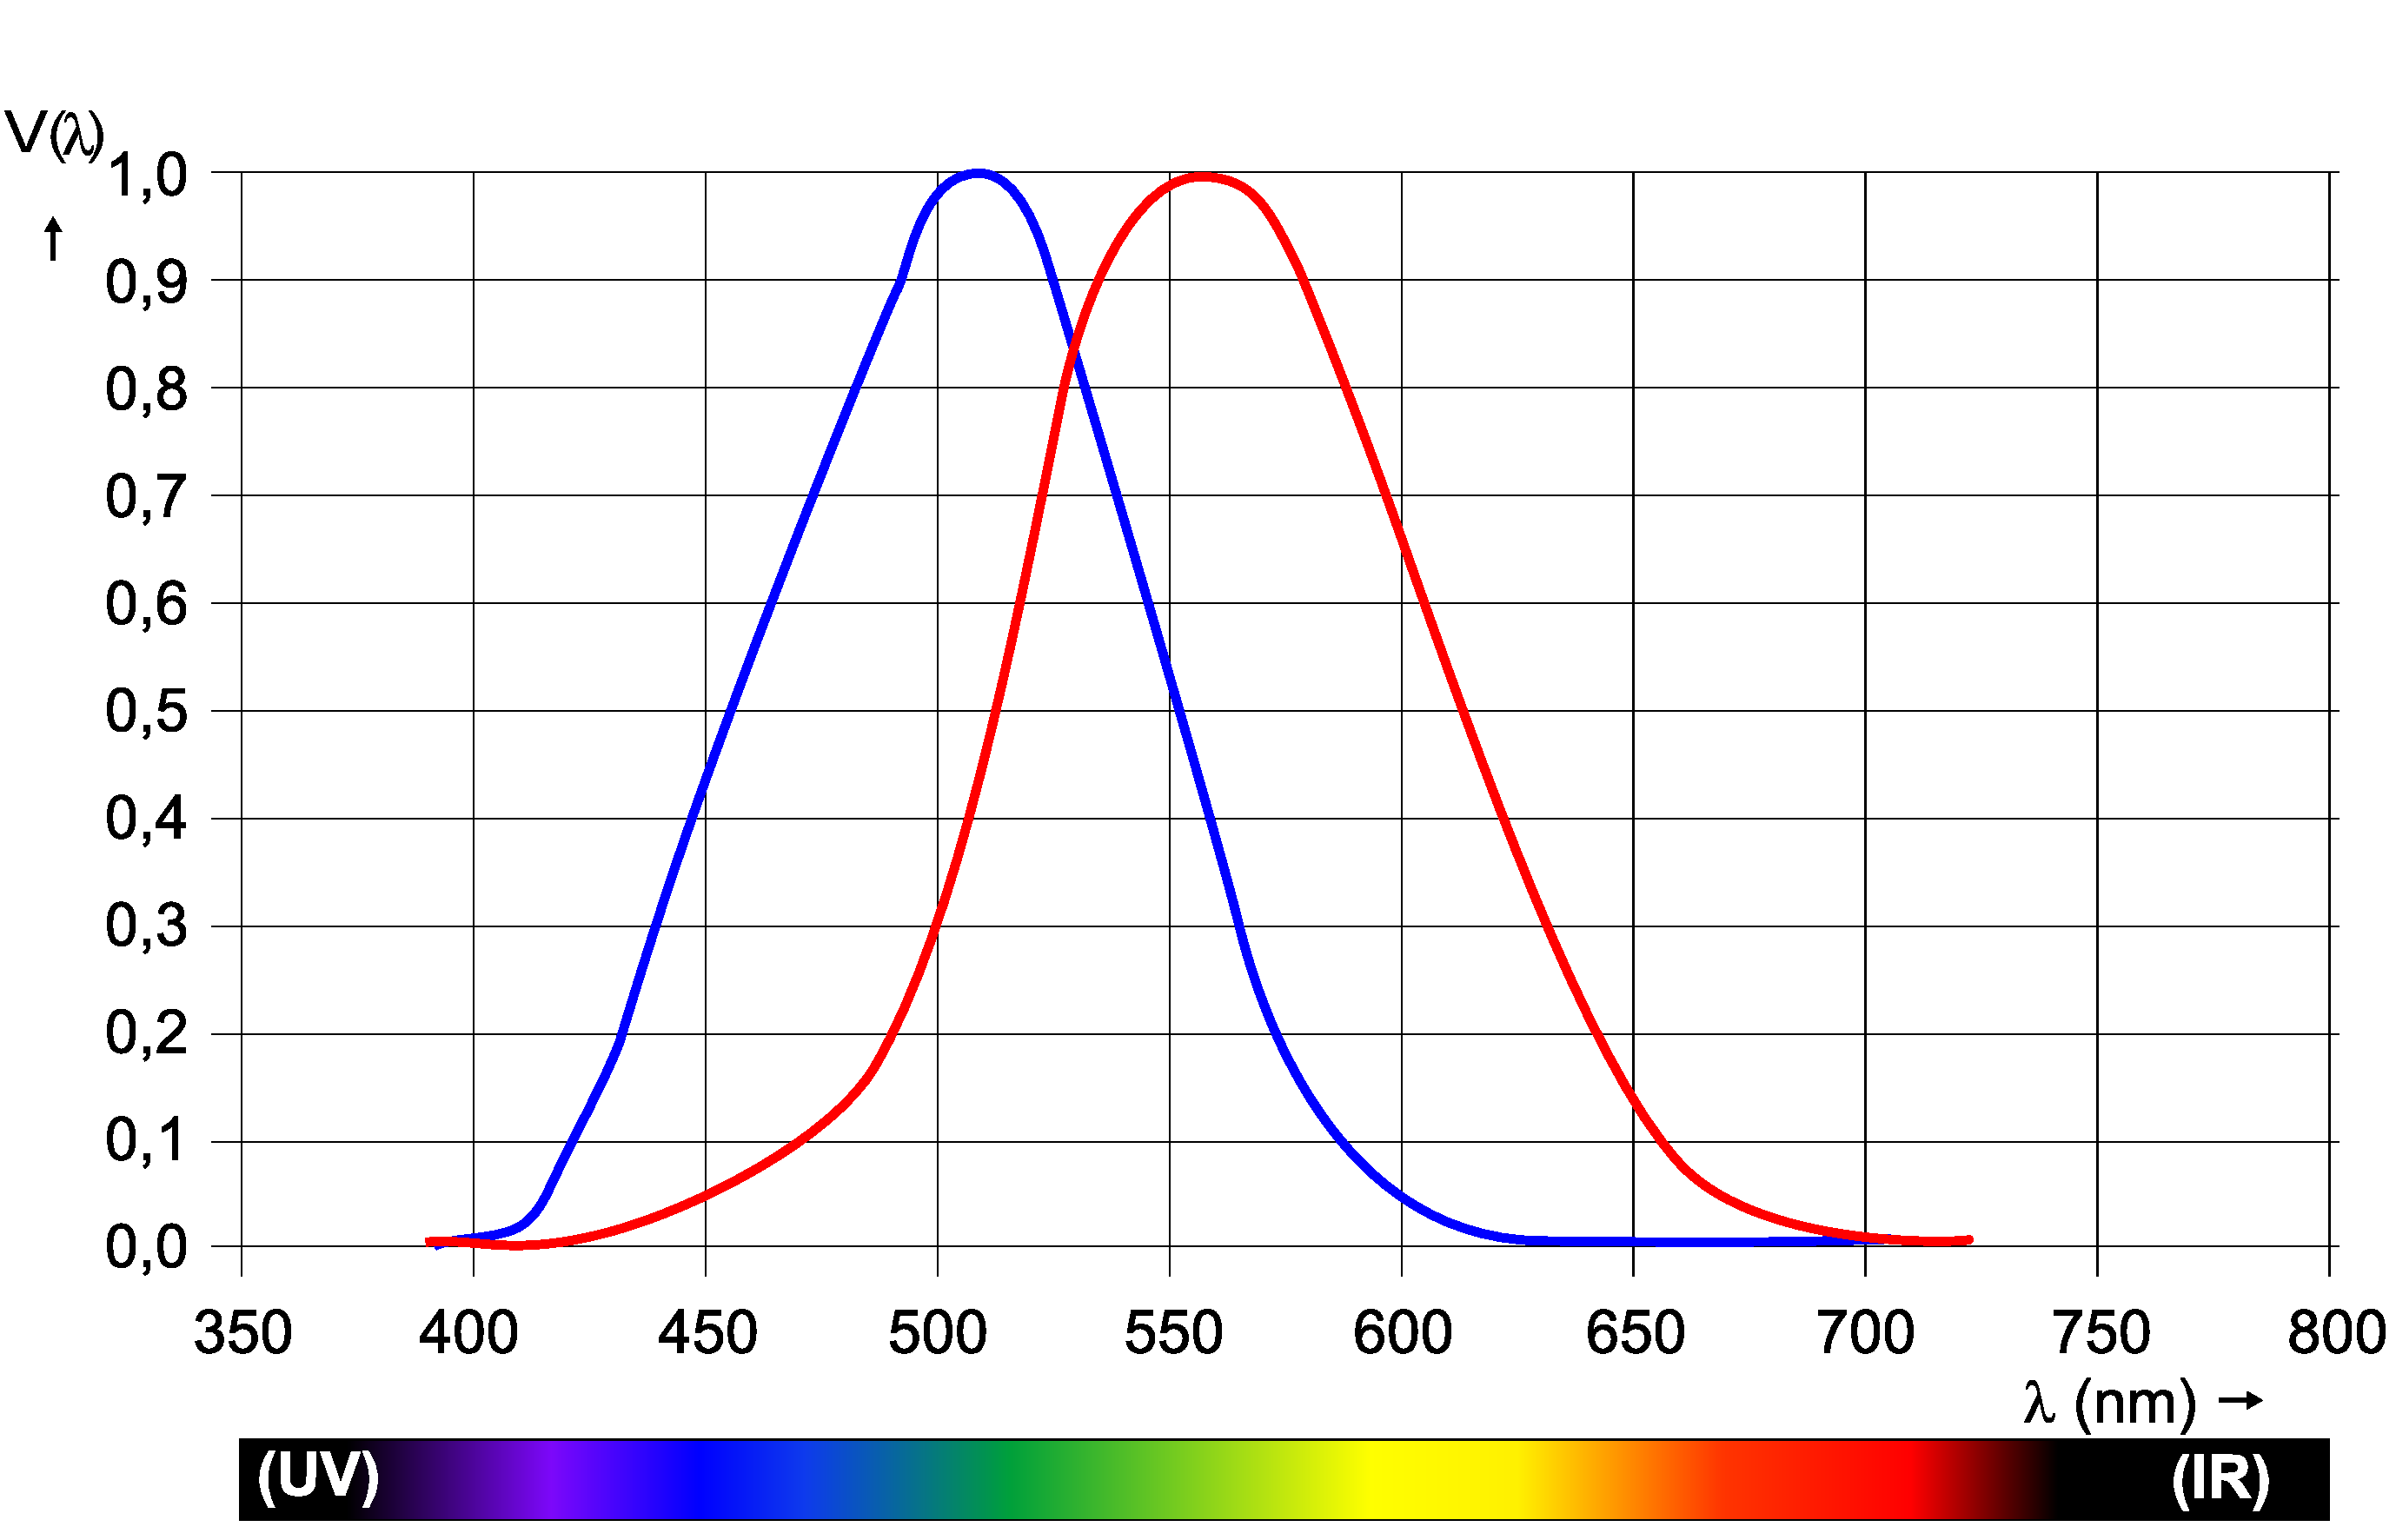
\includegraphics[width=0.5\linewidth]{Bilder/LuminosityCurve1.pdf}
	\caption{CIE Luminosity function V($\lambda$) of the human eye under low light (blue curve) and high light (red curve) conditions \tiny HHahn wikipedia.org \ccbysa}
	\label{fig:luminosity}
\end{figure} 

\subsubsection{Radiant and Luminous flux}

The radiant flux $\Phi_e$ is a scale for the radiant energy Q emitted per time unit on a surface. It is calculated by a given radiant intensity $I_e$ and the solid angle $\Omega$. In other contexts it is also called electromagnetic power: 

\begin{equation}
\Phi_e = \frac {dQ}{dt} = I_e \cdot \Omega ~~ [W]
\end{equation}
\medskip

The complement is called luminous flux $\Phi_v$ in the visible spectrum, with the unit\linebreak lumen [lm]. A light source with 1 cd, that emits in every direction in a solid angle of $4\pi$, will produce a luminous flux of $12.6~lm$. Every material above 0 kelvin radiates light, depending on the surface temperature. The radiated power can be calculated for a ideal black body that absorbs all radiation with the Stefan-Boltzmann-Constant $\sigma$, the material temperature T in kelvin, the emitting area A and the emissivity $\epsilon$ of the surface.

\begin{equation}
\Phi_e = \varepsilon(T)\cdot \sigma \cdot A \cdot T^4  ~~ [W]
\end{equation} 


\subsubsection{Radiant and Luminous Intensity}
 The radiant intensity $I_e$ is used for quantization of the total electromagnetic power emitted by a light source. The power is distributed on sphere areas while moving through space. One steradian (sr) defines an reference area $A=r^2$ on a sphere with the radius r. Figure \ref{fig:steradian} shows the propagation of light under the solid angle $\Omega$.

\begin{equation}
\Omega =\frac {A}{r^2}~~[sr^{-1}]
\label{eq:solid_angles}
\end{equation}

\begin{equation}
I_e=\frac {\Phi_e} {\Omega} ~~ [W sr^{-1}]
\end{equation}
\medskip
\begin{figure}[!h]
	\centering
	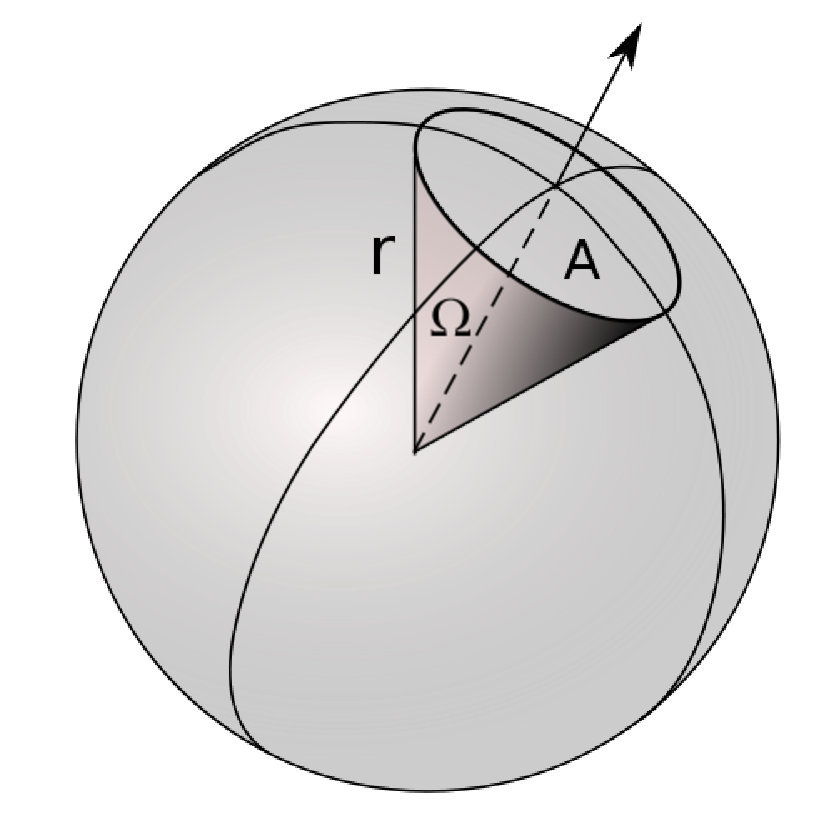
\includegraphics[width=0.3\linewidth]{Bilder/500px-Angle_solide_coordonnees.pdf}
	\caption{Propagation of light in one steradian \tiny Haade wikipedia.org \ccbysa}
	\label{fig:steradian}
\end{figure} 


The radiant power of visible light can be judged by the luminous intensity $I_v$. The power of the spectrum is adapted to the sensitivity of the human eye for different colors. The result is the wavelength-weighted power emitted by the light source per unit solid angle. The unit of luminous intensity is the candela (cd), an SI base unit:

\begin{quote}
	One candela is the luminous intensity, in a given direction, of a source that emits monochromatic radiation of a wavelength of 555 nm and that has a radiant intensity in that direction of $1/683$ watt per steradian\cite{taylor1999nist}.
\end{quote}

A 100 W light bulb offers a luminous intensity of about 1.1 cd. Modern LEDs in contrast can have up to 5 cd, due to the concentration of the emitted light in one direction and a higher luminous efficacy $\eta$ of up to 208 $lm W^{-1}$.

\subsubsection{Luminous Efficacy}
The amount of power P that is transformed in a light source into visible light is represented by the luminous efficacy $\eta_v$. The remaining energy will be radiated in other invisible wavelengths or transferred into a heat flow that vanishes into ambient material and air. 

\begin{equation}
\eta_v = \frac {\Phi_v}{P}
\end{equation}
\medskip

\subsubsection{Radiance and Luminance}
The radiance defined in equation \ref{eq:Radiance_and_Luminance_on_a_surface} is a measure for the quantity of radiation that passes through an area. It can also be used to quantify the amount of radiation, which is reflected from a surface in a specific direction. It changes with the cosine of the incident angle $\varphi$ normal to the emitting surface area. This equation is also called Lambert's cosine law and applies to diffuse reflecting surfaces or Lambertian surfaces.

\begin{equation}
L_e = \frac{I_e}{A_e} = \frac{d^2\Phi_v}{dA~d\Omega~cos\varphi} ~~ [W m^2 sr^{-1}]
\label{eq:Radiance_and_Luminance_on_a_surface}
\end{equation}

\begin{figure}[!h]
	\centering
	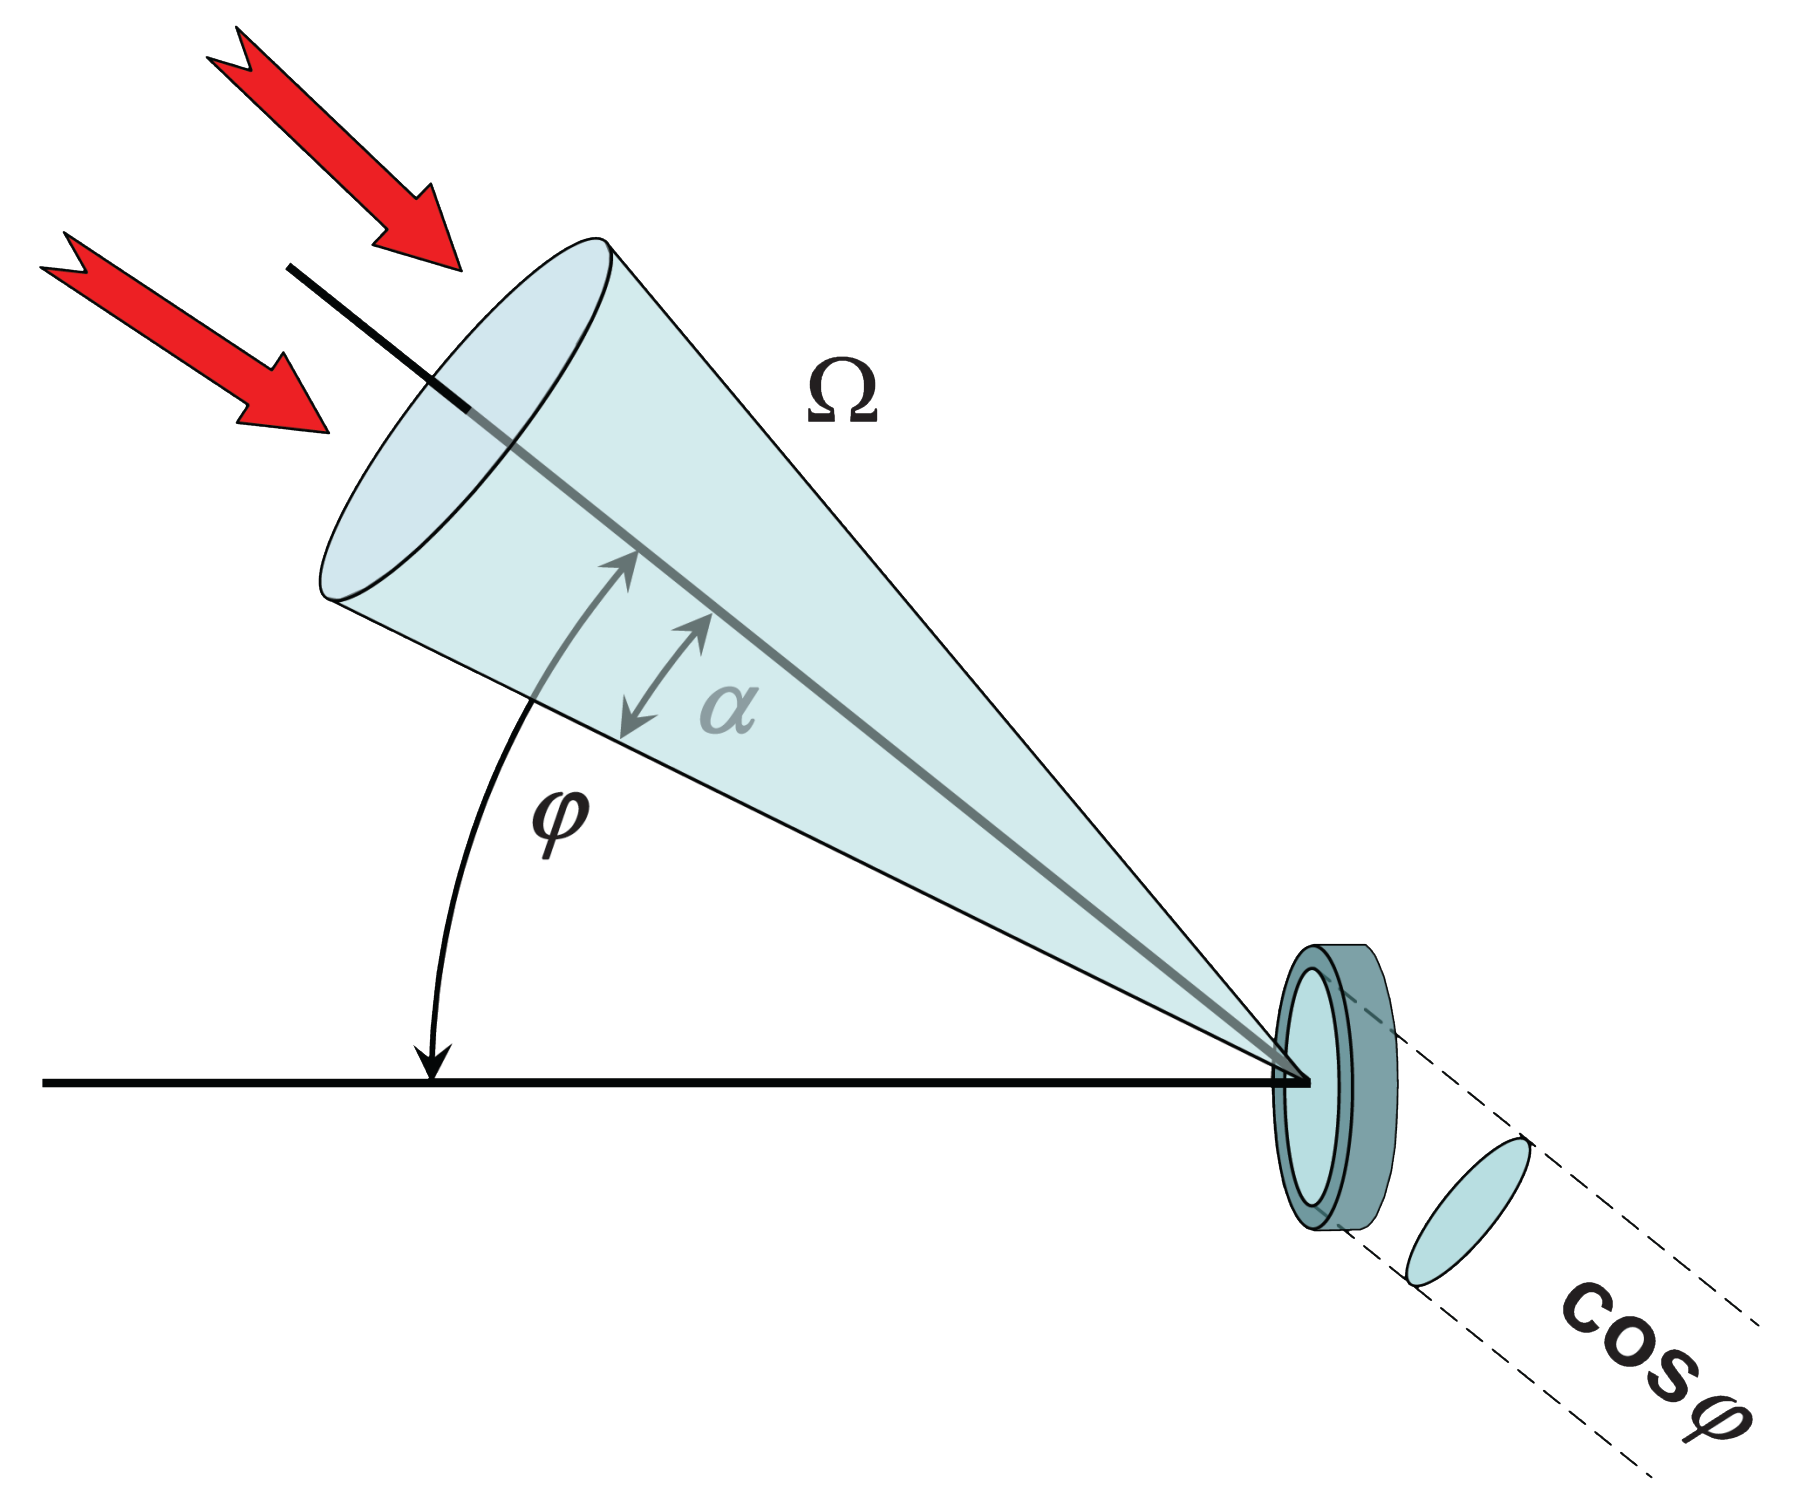
\includegraphics[width=0.4\linewidth]{Bilder/radiance.png}
	\caption{Radiance and Luminance on a surface}
	\label{fig:Radiance_and_Luminance_on_a_surface}
\end{figure} 

The luminance $L_v$ is the analog quantity with respect to the eye. It is a surface's grade of brightness to the human eye.

\subsubsection{Transformation from Radiometric into Photometric}

The radiometric quantities can be transformed into photometric quantities with the help of the Luminosity function V($\lambda$) and the efficacy of radiation $\eta_e$. With a radiant flux given in watt, this value can be compared with photometric quantities in lumen. Even if a light source emits low luminous flux, the destructive impact on the human eye can still be significant from the IR or UV spectrum. That is why for the hazard consideration, the radiometric quantities with specific wave lengths have to be considered. 

\begin{equation}
\Phi_v =\eta_e \cdot V(\lambda) \cdot \Phi_e ~~ [W] 
\end{equation}

\subsection{Diffuse, Spread and Spectral Reflection}

Depending on the wavelength, light interacts differently with material. The surface structure and material properties play a further role in the reflection and absorption characteristics. An ideal spectral reflecting area will radiate all light backwards with the same angle mirrored on the normal vector of the surface. Most materials can give specular reflection, provided that the surface is polished to eliminate irregularities within the magnitude of the wavelength. Transmission is the passage of the electromagnetic waves through a medium. The exit angle of the beam depends on the entry angle and the properties of the medium and light. Diffuse reflection is a combination between transmission and spectral reflection. The waves enter the material and are reflected on the surface multiple times before leaving it again. The direction of reflection is independent from the angle of the incident light. Ideal matt surfaces like white paper have this property and follow the Lambert's cosine law from equation \ref{eq:Radiance_and_Luminance_on_a_surface}. The mixture of diffuse and spectral reflection is called spread reflection and can be observed on most common material. In this case, a diffuse propagation will take place around the direction of ideal spectral reflection, depending on the incident angle \cite{hecht1987optik}. Figure \ref{fig:Diffuse_Reflection} shows the ideal diffuse, spread and spectral reflection of an incident light ray. The reflectivity is the fraction of the reflective $\phi_r$ electromagnetic power to the incident electromagnetic power $\phi_i$.

\begin{equation}
\varrho=\frac{\phi_r}{\phi_i}
\end{equation}

\medskip
 The transformation of radiation in other forms of energy in a medium is called absorption. Heat and other atomic reactions are created by the radiation interacting with the atoms. Some fluorescent materials, like phosphorous, emit the energy over a longer timespan in shifted wave lengths. The ratio of reflectance $\varrho$, transmittance $\tau$ and the absorption $\alpha$ must correspond to the conservation of energy. As a conclusion, equation \ref{eq:Optical_Energy_Convervation} must be fulfilled.

\begin{figure}[!h]
	\centering
	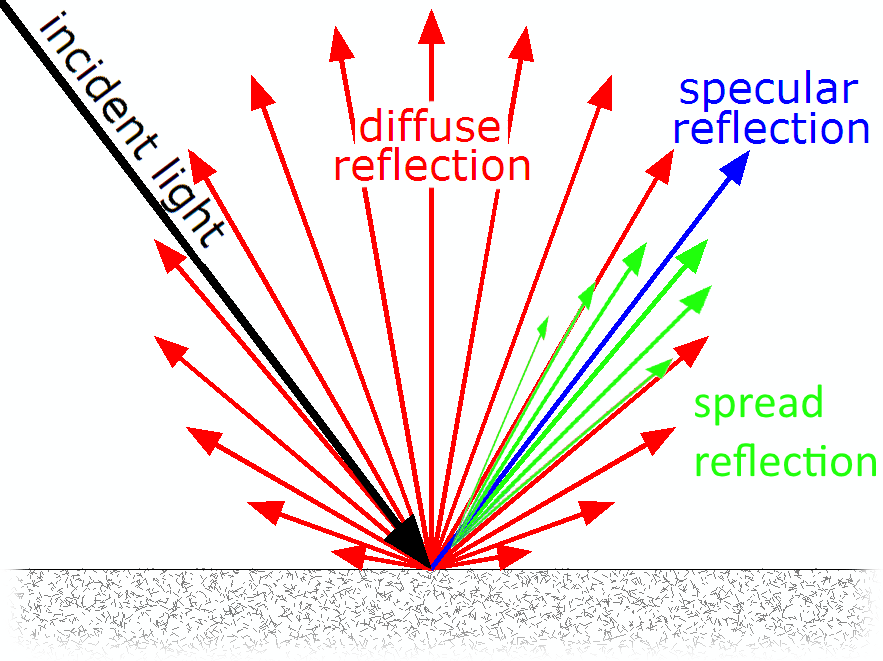
\includegraphics[width=0.4\textwidth]{Bilder/Diffuse_and_Spectral_Reflection.png}
	\caption{Reflection on an ideal mirroring surface and a diffuse surface \tiny GianniG46 wikipedia.org \ccbysa }
	\label{fig:Diffuse_Reflection}
\end{figure} 

\begin{equation}
\varrho +\tau + \alpha=1
\label{eq:Optical_Energy_Convervation}
\end{equation} 
\medskip

The reflectivity depends on the wavelength, the surface structure and the material. Infrared light is reflected in another way than visible light. White paper, for example, is a highly reflecting material for IR light with a reflectance of about $80~\%$. Black paper, in contrast, will absorb most of the incident light. In the reflectance spectrum, the reflectivity is plotted as a function of the wavelength. Aluminum reflects most of the incident light in the IR and VIS spectrum. Gold absorbs most of the radiation in the UV region and becomes reflective for red and IR wavelengths. Figure \ref{fig:Reflection on different metals} shows the reflection versus the wavelength for different metals.

\begin{figure}[!h]
	\centering
	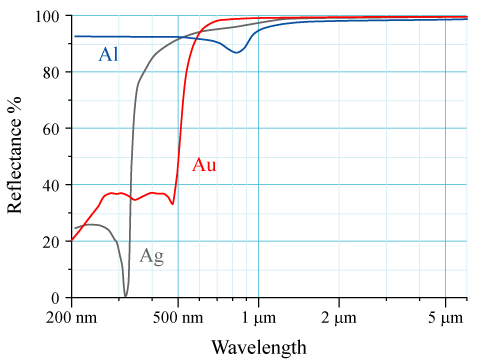
\includegraphics[width=0.5\linewidth]{Bilder/Image-Metal-reflectance.png}
	\caption{Reflectance spectrum of aluminium (Al), silver (Ag) and gold (Au) \tiny Bob Mellish wikipedia.org 2005 }
	\label{fig:Reflection on different metals}
\end{figure} 

\newpage
 
\subsection{Semiconductor Light Sources and Sinks}
 
Nowadays, light generation in semiconductor material plays a crucial role in all regions of illumination. Diodes consist of a chip of two layers of semi-conducting material, which are doped with impurities. As in most diodes, current flows from the anode to the cathode when a threshold voltage $U_{th}$ is reached between both layers. The anode consists of negatively charged holes (p) and the cathode delivers positive charges (n) in form of electrons. The contact area between both materials is called space charge region or depletion area. It gets conductive when the threshold voltage is reached. A current flow in the reverse direction is not possible under normal conditions. Figure \ref{fig:Pnjunction} shows the distribution of impurities in a common diode.
\begin{figure} [!h]
	\centering
	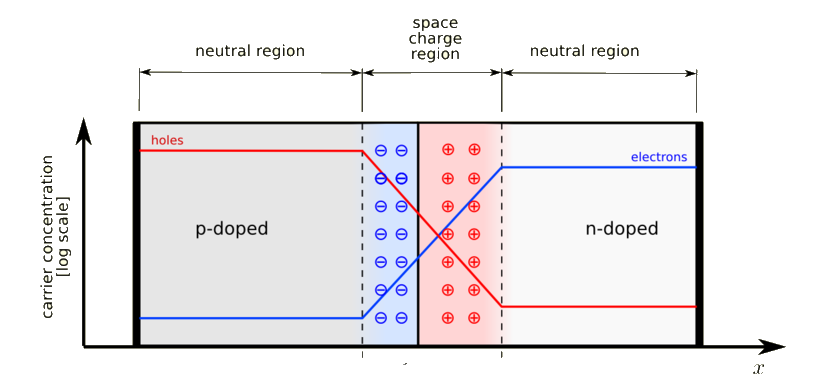
\includegraphics[width=0.6\linewidth]{Bilder/Pn-junction-equilibrium.png}
	\caption{p-n junction of a diode \tiny TheNoise wikipedia.org \ccbysa}
	\label{fig:Pnjunction}
\end{figure}

The recombination of the charges releases energy in the form of radiation. The energy difference between the top of the valence band (holes) and the bottom of the conduction band (electrons) is described by the band gap. The emitted wavelength depends on the size of the gab and the corresponding voltage that drops in this region. For infrared LEDs gallium arsenide (GaAs) or aluminium gallium arsenide (AlGaAs) are used as semi-conducting materials. The emitted wavelength depends on the voltage drop and on the semiconductor material.

A current will flow through a GaAs IR diode at a voltage higher than $1.63~V$. Blue light is emitted from indium gallium nitride diodes and a $U_{th}$ higher than $2.48~V$. This process does also work in the opposite direction. Incident radiation with a wavelength according to the band gap of the diode induces a voltage. In general, this process is possible in every diode, but photo diodes are very sensitive to incident light. That is why this components are used to measure radiation. Figure \ref{fig:thresholdvoltage} shows the current curve versus voltage of an silicon diode. $U_{th}$ is defined as the point with a current flow of $1~mA$. Higher radiant intensity can be achieved through an increase in voltage, which causes a higher current flow \cite{tschirleyelektronik}. With a decreasing temperature, the threshold voltage $U_{th}$ will be shifted to higher values.\\


\begin{figure} [!h]
	\centering
	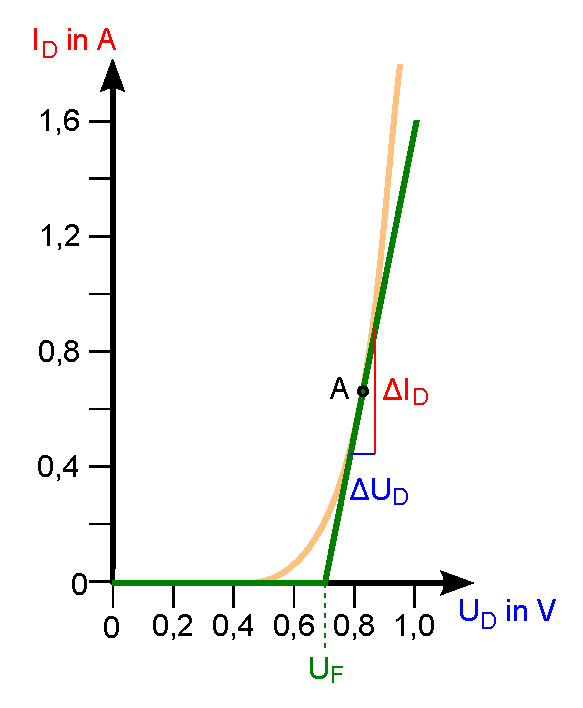
\includegraphics[width=0.4\linewidth]{Bilder/Dioden-Kennlinie_1N4001_differentiell.pdf}
	\caption{Diode current versus voltage \tiny Stuendle 2011 wikipedia.org}
	\label{fig:thresholdvoltage}
\end{figure}

\subsubsection{Light-Emitting Diodes}

With the development of blue LEDs in 1994 new ways of lightning were possible. Other colors, such as red, were discovered in 1968, but only with the discovery of the color blue, the total visible spectrum was covered. The high efficiency and the long lifetime of LEDs offer huge steps in illumination in comparison to light bulbs or halogen bulbs. For the human sensation of white light, another problem had to be solved with LEDs. The color rendering index (CRI) is a measure how the LED reveals the color of illuminated objects in reference to the sunlight. The little fraction of red light in the white spectrum modifies the color of illuminated objects. The light seams to be "cold". More red light on the other hand reduces the luminous efficacy, but increases the CRI value.\\

The electromagnetic spectrum of a LED can be approximated by the Gaussian distribution. A blue LED will emit light with wavelengths between 450 and 500 nm. This range is called spectral width. The speed of respond is often given by the rise and fall time; the time required to go from  $10~\%$ to $90~\%$ power. The shortest possible pulse length with modern fast LEDs can be shorter than $1~ns$. As a conclusion results the maximum switching frequency can be up to multiple megahertz for LEDs.\\   
White light can be generated by the combination of red, green and blue. Another method is the coating of a blue LED with phosphor: A fraction of the blue light undergoes a wavelength shift, being transformed from shorter to longer wavelengths.\\

There are two basic types of LED structures: Edge emitters and surface emitters. Surface emitters have a comparatively simple structure. The light will be radiated in all directions from the surface of the semiconductor. The total optical output power is higher than the one from edge emitters. In contrast, edge emitters have a smaller spectral width, a very high power density and a internal optical gain like a laser. The light leaves the chip between the layers on the edge of the semiconductor \cite{botez1979comparison}.\\

The normalized radiant intensity as function of the angle of radiation can be determined experimentally and characterize from different angles. These diagrams are often published by manufacturers in the data sheets of the light source as shown in figure \ref{fig:radiation_diagram} for a common IR LED. \\

\begin{figure} [!h]
	\centering
	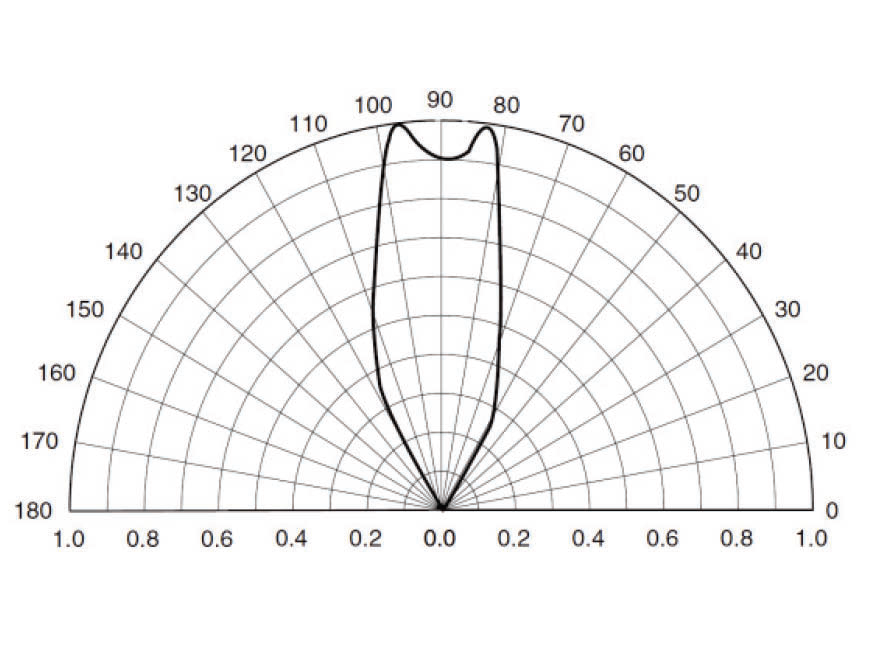
\includegraphics[width=0.5\linewidth]{Bilder/radiation_diagram.png}
	\caption{Radiation diagram of a IR LED \tiny QED222 www.fairchildsemi.com}
	\label{fig:radiation_diagram}
\end{figure}

\newpage

\subsubsection{Laser Diodes}
Laser diodes in contrast to LED create monochromatic light in a narrow bandwidth. An additional undoped intrinsic semiconductor is implemented between the p-n junction. It emits light waves with  chronologically steady polarization and phases to each other. Therefore, ideally only a fixed wavelength is created. As a conclusion the oscillation of the emitted light is therefore phase-synchronous. The beam deivergence is low. This property is called collimated in optics \cite{thompson1980physics}. An important advantage of laser diodes is the fact, that it can be modulated in intensity with high frequencies up to several gigahertz and extreme short pulses in the region down to femtoseconds. In most technical implementations, the laser light intensity will be additionally measured with a photo diode near the laser diode to get a feedback for precise control. Unlike a regular diode used in electronics, the goal for a laser diode is that all carriers recombine in the I region, and produce light. Thus, laser diodes are fabricated using direct bandgap semiconductors. Figure \ref{fig:laserdiode} illustrates the setup of a laser diode on its heat sink, the monitoring photo diode and the protecting window.

\begin{figure} [!h]
	\centering
	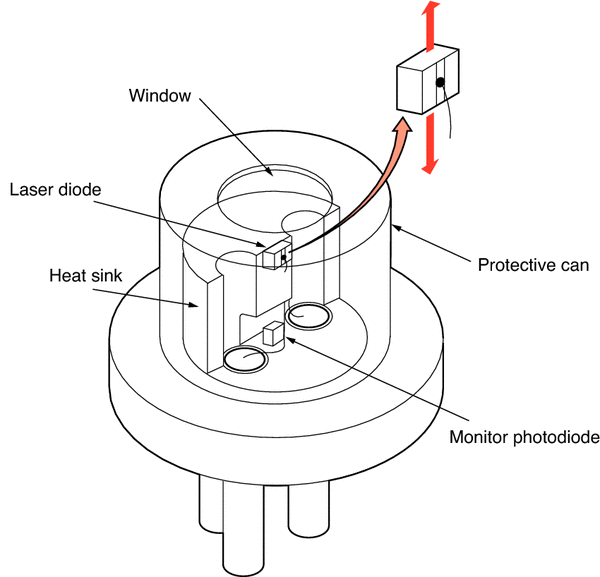
\includegraphics[width=0.5\linewidth]{Bilder/laser_diode.png}
	\caption{Setup of a common laser diode \cite{newport}}
	\label{fig:laserdiode}
\end{figure}

\subsubsection{Photo Diodes} 
Photo diodes are used for the conversion from radiant into electrical energy. The physical principle behind this is the inner photoelectric effect. If absorption of light occurs in the junction, holes move to the anode and electrons to the cathode. A current is induced and therefore a voltage can me measured. The responsivity $R_\lambda$, also known as responds, is the ratio between the current flow relative to the radiant power in different wavelengths. The quantum efficiency (Q.E.) is defined as the fraction of the incident photons, that contribute to photo current.

\begin{equation}
R_\lambda = \frac{I_P}{P} ~~ [A W^{-1}]
\end{equation}

\begin{equation}
Q.E. = R_\lambda \cdot \frac {h c} {\lambda q}~~[1]
\end{equation}

\begin{figure} [!h]
	\centering
	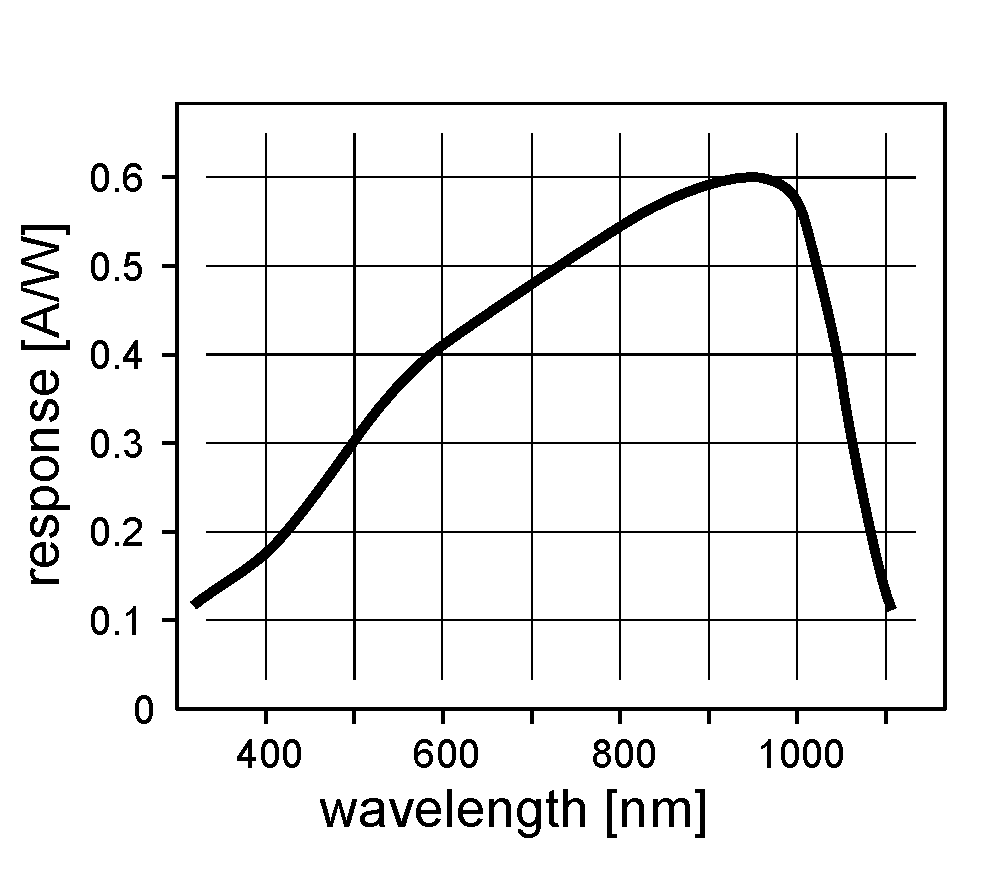
\includegraphics[width=0.5\linewidth]{Bilder/Response_silicon_photodiode.pdf}
	\caption{Response over wavelength of a silicon photodiode \tiny Kai Martin 2007 wikipedia.de \ccbysa}
	\label{fig:response}
\end{figure}

Every signal of the photo diode will be overlayed by dark current and thermal current. This noise results from electromagnetic background radiation and thermal movement of the charge carriers. To achieve the raw noise characteristics of a photo diode, the output signal must be measured in an absolute dark room with no background radiation. 

The rise and fall time of a photo diode can be expressed as the frequency response at which the output amplitude decreases by $3~dB$. Three factors influence the response time:
\medskip \\
\begin{enumerate}
\setlength\itemsep{0.001em}
\item The charge collecting time of the carriers in the depleted region. 
\item The charge collecting time in the undepleted region.
\item The resistance and capacity of the diode circuit combination.
\end{enumerate}

\begin{equation}
t_r \cong \frac{0.35}{f_{3dB}}~~[s]
\end{equation}
\medskip

Single-photon avalanche diodes (SPAD) are very sensitive to incident light and enable the measurement of very low intensities. The electric field between the junction is so high, that the arrival of a single photon can be determined down to ten picoseconds. A photo-generated carrier triggers an avalanche current due to the impact of ionization mechanism. The circuit behind the diode must fulfill multiple tasks \cite{cova1996avalanche}:

\begin{enumerate}
	\setlength\itemsep{0.001em}
	\item Sense the leading edge of the avalanche current. 
	\item Generate a standard output pulse synchronous with the avalanche build-up.
	\item Quench the avalanche by lowering the bias down to the breakdown voltage.
	\item Restore the photo diode to the operative level.
\end{enumerate}

\subsection{Image Sensors}
A radiant flux can be converted into a 2D data matrix by an image sensor, an array of photo diodes. Every single element of the array, a so-called pixel, consists of one or multiple photo diodes, that are arranged in columns and rows. The pixel pitch is the dimension of a single pixel. The area that is actually sensitive to the light is determined by the fill factor times the pixel pitch. Without a micro lense, this area corresponds to the photodiode surface. The physical extent of the complete flat sensor is called optical size. An ordinary picture of visible light consists of a mixtures of red, green and blue (RGB) colors, but single photo diodes can only be optimized for a narrow band in the light spectrum. The band gap must correspond to the wave length of the light to detect it. Therefore three diodes are needed to deliver the RGB information on one pixel. They can be arranged side by side or stacked. The classical Bayer filter separates the light with red, green and blue filters. Foveon X3 sensors, in contrast, use three stacked photo diodes with various band gaps. IR image sensors are made of special semiconductor material like Indium Gallium Arsenide. 

\subsubsection{Charged-Coupled Device Sensor}

The first digital image sensor was based on the charged-coupled device (CCD) architecture. In the first place Bell Labs invented this type of integrated circuit for data storage in shift register. Charges could be shifted between the different capacitors that hold the energy of each diode. Later, it was discovered that this circuit can also be used as an image sensor. After the array is exposed to light, every pixel contains information about the incident light in form of charges. This data is transferred into a storage pixels array. Gathered charges are transformed into a corresponding voltage by a single amplifier in series order. The signal can be converted afterwards into a digital representation or into a continuous analog signal. The bit depth or color depth of the analog-to-digital converter (ADC) is given in bits and specifies the number of possible steps for the discretization. The color precision depends on this value and on the amplifier characteristics.


\subsubsection{Complementary Metal-Oxide-Semiconductor Sensor}

Modern semiconductor technology lead to the development of image sensors that are produced based on complementary metal-oxide-semiconductors (CMOS), also called active-pixel sensor. In contrast to CCD, every pixel is implemented with his own amplifier. Other components, like the ADC or the oscillator are integrated onto the sensor chip. This allows production under a much lower cost. Thus most consumer market cameras nowadays are based on this technique. The simplest realization of an CMOS pixel can be done by a photo diode and three CMOS transistors as shown in figure \ref{fig:CMOS_architecture_storage_pixels}. The charges will be gained inside every pixel after the exposure time. The circuit can be discharged via the reset connection, for every new image.

\begin{figure} [!h]
	\centering
	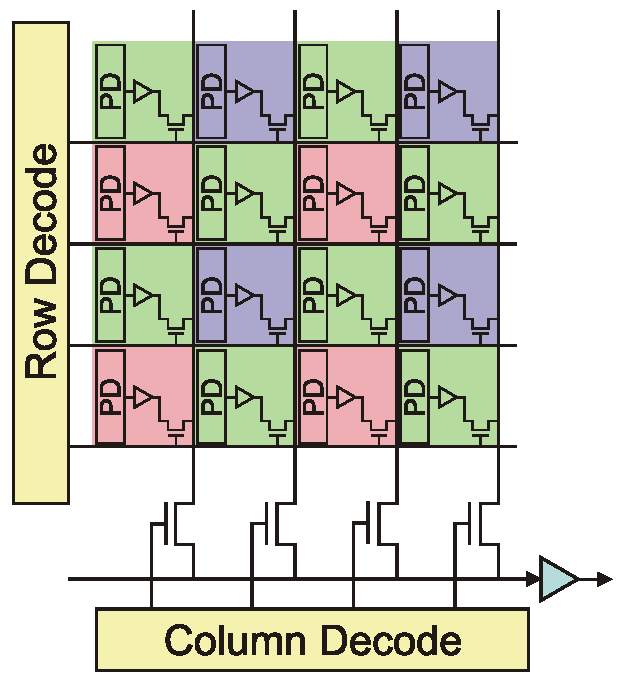
\includegraphics[width=0.4\linewidth]{Bilder/CMOS_Image_Sensor_Mechanism_Illustration.pdf}
	\caption{Frame transfer in a CMOS image sensor \tiny Shape 2008 wikipedia.de}
	\label{fig:CMOS_architecture_storage_pixels}
\end{figure} 

\newpage
\subsubsection{Attributes of Image Sensors}
For the foreseeable future, CCD and CMOS sensors will play both a significant role in imaging procedures. The long experience with CCD sensor production and the associated reliability is one of the major advantages in comparison to CMOS for scientific applications. Nevertheless, CMOS technology gains growing interests for scientific applications with developments driven by the consumer market. The following attributes are used to differ between the characteristics of both images sensors \cite{neugebauer1991parallel} \cite{litwiller2005cmos}.\\
     
\textbf{Dynamic Range}\\
The ratio between the saturation of a pixel to its threshold to detect photons is called the dynamic range (DNR). Saturation is reached when additional light will not cause more charges. The DNR is often represented in decibel. A low threshold is only possible with a low Signal-to-Noise Ratio (SNR). It describes the power ratio between the signal that needs to be measured and the unwanted background noise \cite{bushberg2011essential}. 

\begin{equation}
DNR = 20\cdot\log{\frac{P_{saturation}}{P_{threshold}}}
\end{equation}

\begin{equation}
SNR = \frac{P_{signal}}{P_{noise}}
\end{equation}
\medskip

The human eye has its highest dynamic range in the green spectrum. It enables us to see very small differences in color and brightness in this range. The contrast radio describes the same property for display systems. A high contrast radio is desired for most displays. Small shades between colors can be distinguished better.\\  

In the past CCDs enjoy significant noise advantages over CMOS because of less circuits on the chip that interfere the measurement. ADCs and other components are outsourced from the image sensor. This issue has been solved by the development of modern CMOS and the possibility to integrate the signal processing at the sides of image sensor, which has substantially dampened many noise sources and improved CMOS performance.\\ 

\textbf{Uniformity}\\
Ideally, every pixel should behave in the same way under identical illumination conditions. In practice, inaccuracies in the semiconductor production cause small variance in the structure of the photo diodes. This problem occurs with CCD and CMOS. CCDs benefit from the single amplifier, that every charge goes through. As a conclusion all values are increased with the same gain. In CMOS variations between the amplifier causes a higher uniformity. This is a significant issue in high-speed applications with a limited SNR. The short exposure time gathers only small amounts of charges. Consequently uniformity between the pixels will emerge under the short exposure time.\\   
  
\textbf{Speed}\\
The highly integrated CMOS technology makes this type of sensor much faster than CCD. Capacitance and propagation delays are shorter, because the circuitry is integrated into the chip. The charge transfer time is much shorter and the ADC processing can be done directly in the image sensor. This results in much higher speeds with CMOS. Images can be made in a very short distance to each other. Therefore, CMOS allows higher frames-per-second (fps). \\

\textbf{Windowing}\\
One limitation for the maximum speed of a camera is the ability to transfer and save all captured images. CMOS sensors allow the independent operation of parts on the image sensor. The number of working pixels is decreased to increase the maximum possible speed between every capture. This function is called region-of-interest (ROI) or windowing in modern industrial cameras.\\

\textbf{Antiblooming}\\
Blooming is the unwanted movement from charges between pixel in saturation. CMOS is immune for this effect, because every pixel is separated from each other. Modern CCD reduce this effect with the help of Anti-Blooming Gates. Unfortunately, this limits the size of the pixel and therefore the dynamic range.  

\subsubsection{Rolling and Global Shutter}
In traditional analog photo cameras, the shutter speed is the time in which the film is exposed to the light. The shutter opens and closes mechanically. The time in between is also called exposure time $t_e$. Today this is done without any mechanic in a digital camera. The sensor starts, stops and resets based on a digital control signal. Two different types of electronic shutters can be distinguished. The rolling shutter is used in most CMOS consumer cameras. The rows of the image sensor start their measurement shifted to each other. This causes the rolling shutter effect when fast moving scenes are measured in the order of the exposure time or smaller. The time delay between the lines can produce a blur in the picture. This kind of shutter is not desired for scientific and industrial investigations of fast moving objects. Figure \ref{fig:Rolling_shutter} shows the timing of a rolling shutter image sensor. 

 The global shutter is used in most scientific and industrial cameras. Every row of the image is exposed at the same time without any phase shifting. In the past, this was one of the main benefits of CCD cameras. New developments allow the combination between global shutter and CMOS. Figure \ref{fig:Global_shutter} shows the timing of a CMOS global shutter camera. Images can be captured without geometric distortions. A longer readout time is necessary for the processing of charges in parallel. The camera is "blind" in this time slot for incident light. A flashlight synchronized to the camera trigger is a indicator that is commonly used to investigate the shutter of the camera. A trigger input or output at the camera allows the synchronization of the image exposure to the flash or other devices. The camera and the lighting can be shifted to each other to evaluate the timing of the reset, exposure, readout and charge transfer. For the synchronization between multiple cameras, the trigger channel enables the fixed phase relation between images from different perspectives. This is especially necessary when dynamic processes are investigated. The exposure time $t_e$ must always be smaller than the frame periode. Consequently, the exposure time must be reduced with higher frame rates (fps):
 
 \begin{equation}
 t_e < \frac{1}{fps}
 \end{equation}
 \medskip

\begin{figure} [!h]
	\centering
	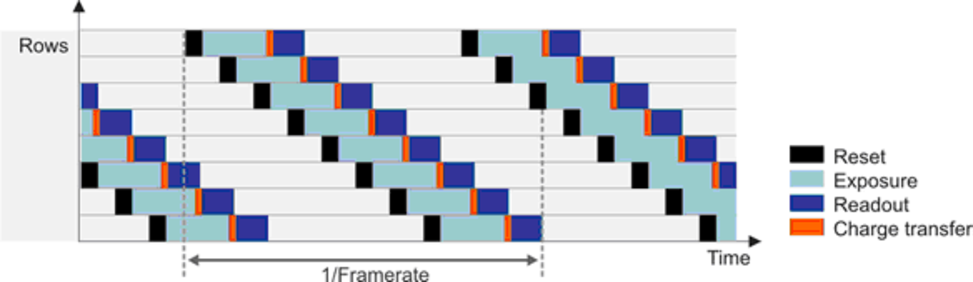
\includegraphics[width=0.6\linewidth]{Bilder/rollingshutter.pdf}
	\caption{Timing of rolling shutter CMOS Sensor \tiny http://www.cihansari.com/}
	\label{fig:Rolling_shutter}
\end{figure} 

\begin{figure} [!h]
	\centering
	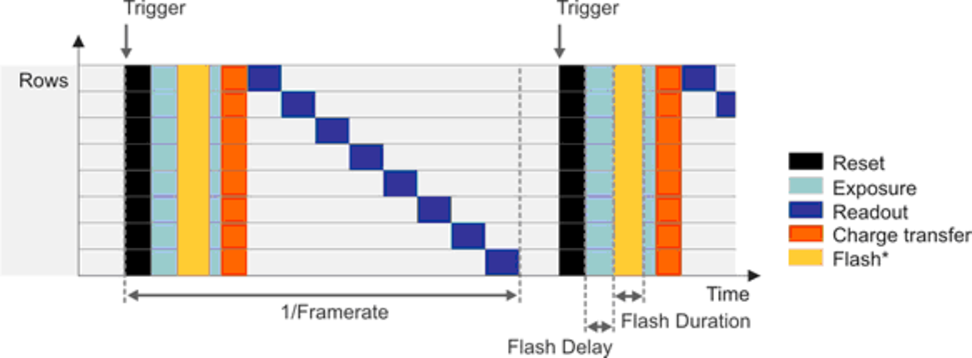
\includegraphics[width=0.6\linewidth]{Bilder/globalshutter.pdf}
	\caption{Timing of triggered global shutter CMOS sensor \tiny http://www.cihansari.com/}
	\label{fig:Global_shutter}
\end{figure}  

\subsubsection{Camera Optic} 
The image sensor without a lens in front of it is not able to capture a sharp image. The ambient light from different angles will overlap on multiple pixels. That is why a lens is needed to direct the path of the light rays as parallel as possible on the sensor. Every point of the scene should ideally be represented on the image sensor only on one position. For different distances this is not possible with a fixed lens position. A focus is needed to change the plane of the lens and therefore the focal length $F$. As a consequence the plane in which the scene is captured sharply is moved. Figure \ref{fig:focal_length} shows some basic dimensions of the camera optic. With a higher maximum $F$, sharp pictures can be made from a long distance $d$. The angle of view $\theta$ is reduced in contrast. The focal length is a scale for the optical power of a lens and to measure how strong the rays are bended. The optical axis stands normal to the middle of the image plane and point into the middle of the investigated scene. 
\begin{figure} [!h]
	\centering
	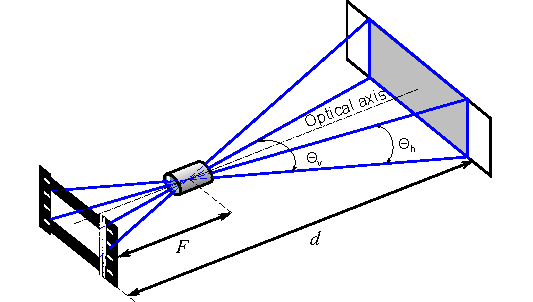
\includegraphics[width=0.5\linewidth]{Bilder/angle_of_view_3d.pdf}
	\caption{Focal length in the camera optic \tiny Christophe Dang Ngoc Chan 2007 wikipedia.org \ccbysa}
	\label{fig:focal_length}
\end{figure}  

The field of view (FOV) is the image section of the scene that is observed. In an optical instrument it describes the solid angle through which a detector is sensitive to incident electromagnetic radiation. The aspect ratio of the resulting images corresponds to the aspect ratio of the field of view. It can be calculated by the vertical and horizontal angle of view $\theta_{v,h}$, as described by equation \ref{eq:aspect_ratio}.

\begin{equation}
\label{eq:aspect_ratio}
Aspect~Ratio = \frac{\tan({\theta_v})}{\tan({\theta_h})}
\end{equation}

 The lens speed N is the ratio between the maximum possible aperture and the focal length of the objective. The illuminance, that can be captured by the lens, increases with the square of the aperture. A lens with a larger maximum aperture is called a fast lens because it delivers more light in the same exposure time.
 
\begin{equation}
N=\frac{F}{D}
\end{equation}

\subsubsection{Motion Blur}
Motion blur occurs when the sensor or an object in the scene moves within the exposure time of an image. One observed point will be projected to multiple positions on the image sensor. This can be avoided with a very short exposure time $t_e$ or with a stroboscope in a dark room that controls the amount of light in the scene. The movement $\vec{s}_{blur}$ of every point inside a picture can easily be calculated when the velocity $\vec{v_p}$ parallel to the picture plane is known and constant.

\begin{equation}
{\vec{s}_{blur}} = \vec{v_p}\cdot t_e ~~[m]
\label{eq:motion_blur}
\end{equation}

Figure \ref{fig:motionblur} shows the motion blue on a propeller. The speed on every point on the blades $\vec{v}$ can be calculated with angular velocity $\vec{\omega}$ and the radius $\vec{r}$ to the axis of rotation. The velocity $\vec{v_p}$ is the projection of $\vec{v}$ on the image plane. The blur increases linear with the radius to the axis.

\begin{equation}
\vec{v} = \frac{d\vec{r}(t)}{dt} = \vec{\omega}\times \vec{r}~~[ms^{-1}]
\end{equation}

The scalar angular velocity can be calculated by the rotational speed n. With the axis of rotation as z the vectorial angular velocity can be derived. This can also be used to calculate the rotational speed from a blurred picture with known exposure time and geometry of the rotor. 


\begin{figure} [!h]
	\centering
	\fbox{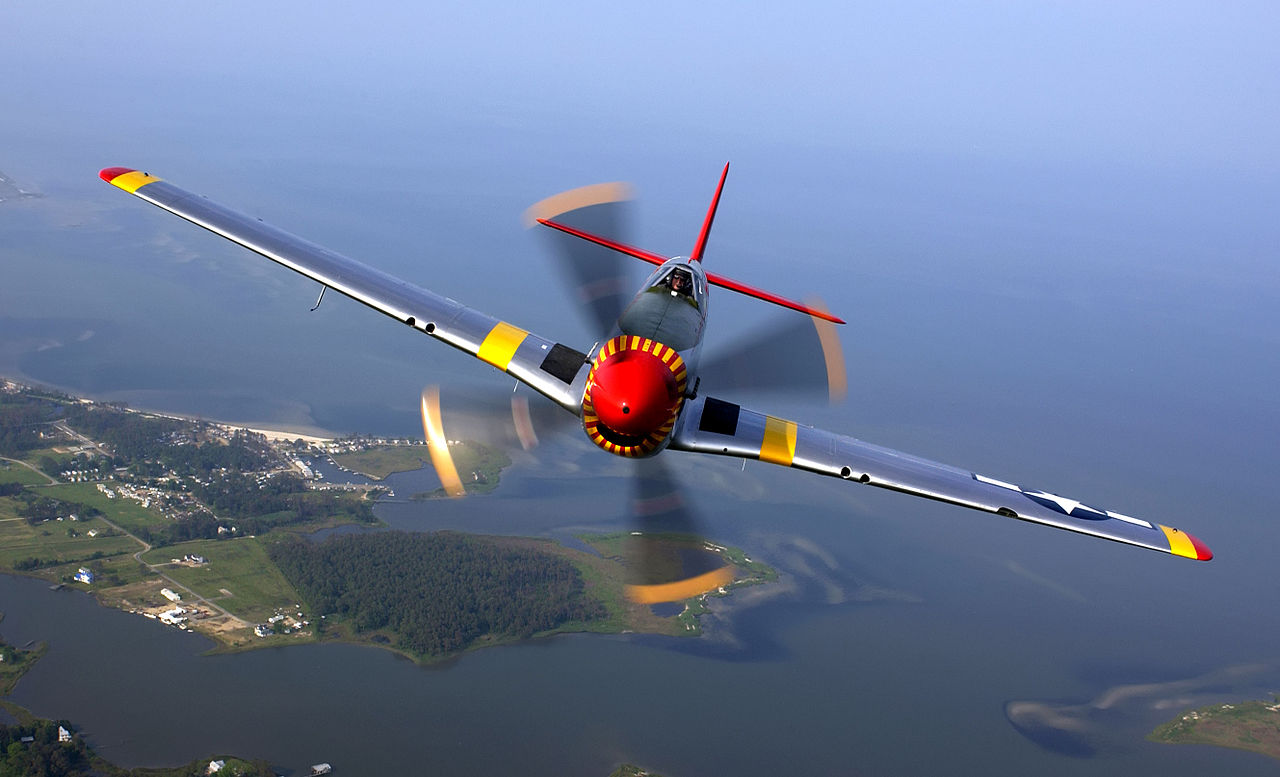
\includegraphics[width=0.45\linewidth]{Bilder/P-51_Mustang_edit1.jpg}}
	\caption{Motion blur of a fast moving rotor \tiny Tech. Sgt. Ben Bloker wikipedia.org}
	\label{fig:motionblur}
\end{figure} 

\newpage

\subsection{Range Imaging Techniques}
Multiple 3D scanning approaches are used, to derive three-dimensional data from the real world. In this section, a comparison of different range imaging techniques and their characteristics is done. They all produce 2D images, that represents the distance to every point in the scene, a so called range or depth image. This data can be transformed into a 3D space, when the system is calibrated adequately to the field of view, which depends on the focal length or freedom of movement of the laser. Various methods have been developed, to determine the distance to the image sensor.


\subsubsection{Stereo Triangulation}
The position of a point in space can be reconstructed from the perspective of two or more cameras. This requires a calibrated position and field of view of the cameras to each other. With two images of the same scene, taken from different points of view, the correspondence problem has to be solved. It describes the challenge of finding a set of points in one image, which can be identified as the same points in the other image from a different point of view. Two basic methods are distinguished:\\

\textbf{Correlation-based} - Check if identical location can be found in both images.\\
\medskip
\textbf{Feature-based} - Find multiple features in the images and see if a layout of subsets is similar.\\

\begin{figure} [!h]
	\centering
	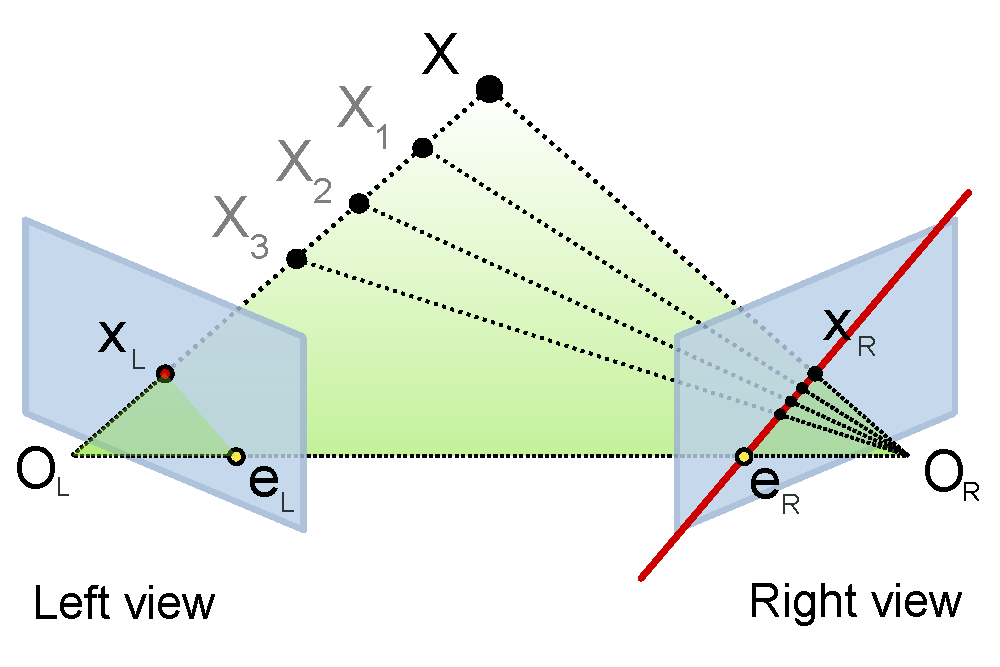
\includegraphics[width=0.6\linewidth]{Bilder/Epipolar_geometry.pdf}
	\caption{Basic principles of stereo triangulation \tiny Arne Nordmann 2007 \ccbysa }
	\label{fig:stereovision}
\end{figure} 

Markers are easy additives to identify single points from multiple perspectives. Figure \ref{fig:stereovision} shows one scene that is observed from two position. The point $X$ is projected as $X_R$ and $X_L$ on both image sensors. The epipolar line between $O_L$ and $O_R$ is the base for the triangulation \cite{finsterwalder1897geometrischen}. The position of the point X cannot be distinguished in the depth with just the left image. With the second image, the range of every point can be calculated. The nearer the objects are to the image sensor, the higher  the displacement of the object between the two images is. Therefore, the triangulation is simplified and more accurate. The human eyes work by the same principle to determine the depth in the human field of view. The basic principle is also called stereo vision and allows the measurement of distances down to $10^{-7}~m$ \cite{thierryoggietof}.


\subsubsection{Structured Light Sensor}
The projection of a structured light pattern is an established method to derive the depth of a scene into the room and to analyze it by a camera. The orientation of the camera and the lighting projection must be known to reconstruct the 3D surface from the 2D picture. The light pattern is created by interfering of two coherent laser beams or by a display that is projected. From the perspective of the camera, the pattern is deformed by the 3D surface. The new distribution is the base for the depth reconstruction. In most technical implementations, the wavelength of the light can be found in the IR spectrum. The human eye cannot see the structure. The measurement will be disturbed by surfaces that absorb or spectral reflect. Ideally, the light reflects in a diffuse way from the surface. Figure \ref{fig:Kinect1_structured_light} is an image of the point structure that is projected on a model aircraft with a Kinect 1 camera. From that, the raw uncalibrated depth image is calculated where every pixel corresponds to a value of one depth measurement. The vertical stabilizer at the rear end cannot be acquired, because it lies under the minimal distance of about $0.8~m$. A hole seams to appear in this region. One major disadvantage is the low range of structured light sensors. Thus, most implementations are in the close-up range for applications, like gesture recognition. An enhancement of this method is the Programmable Structured Light (DLP). The light pattern can be adapted onto the target object to capture physical measurements, analyze locations or inspect a surface.

\begin{figure}[!h]
	\subfigure[IR point pattern]{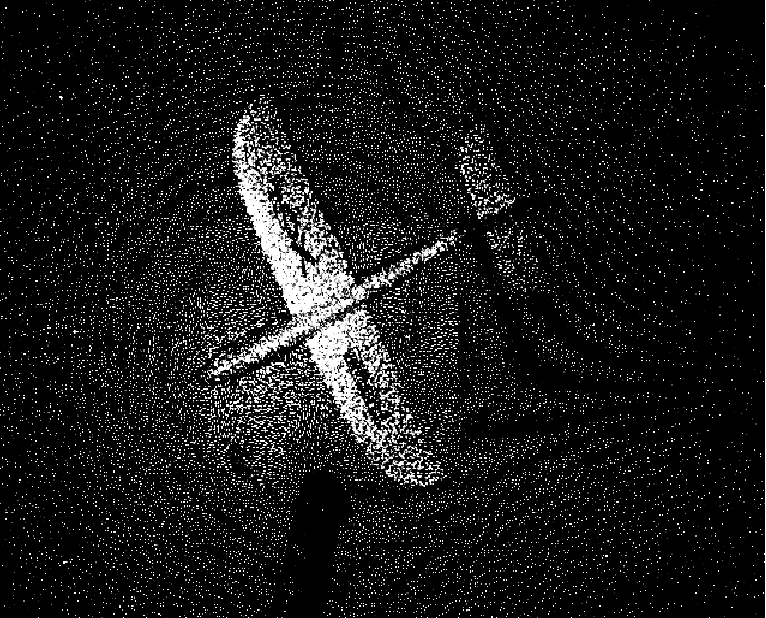
\includegraphics[width=0.45\textwidth]{Bilder/IR_Pattern.png}}\hfill
	\subfigure[Depth data resulting from the IR image]{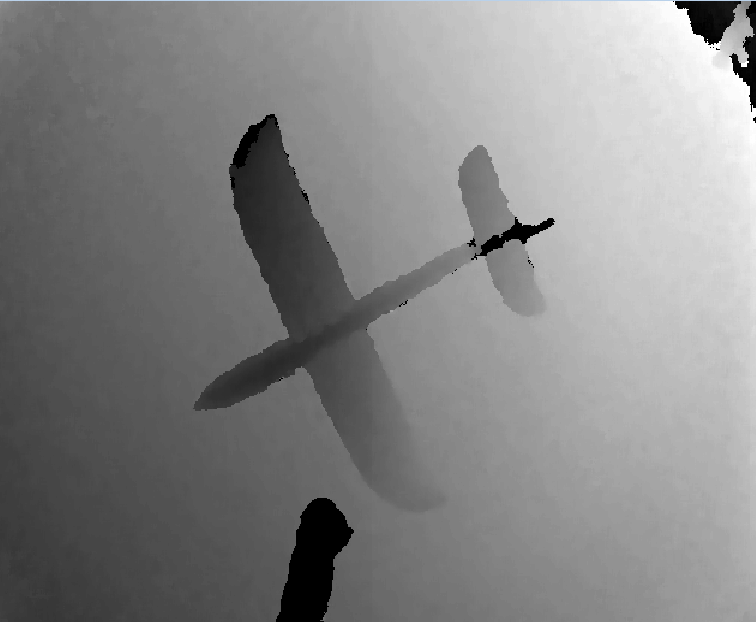
\includegraphics[width=0.45\textwidth]{Bilder/depth_pattern.png}}
	\caption{Kinect 1 structured light}
	\centering
	\label{fig:Kinect1_structured_light}
\end{figure}
\newpage

\subsubsection{Interferometry}
The Doppler effect is the change in frequency that occurs when the observer moves relative to the wave direction. In the interferometry this effect is used to measure the absolute velocity $v$ of an objects relative to stationary coherent light sources with a constant frequency $f_E$. The interference between the reflected and the emitted light results in a new waveform. The interfering light has the new frequency $f_D$ that is proportional to the speed $v$ of the reflecting body. A photo diode measures the sum of the spectral components $f$ and can therefore calculate the frequency shift \cite{CLVpolytec}.

\begin{equation}
f= f_D \pm \frac{1}{\lambda}
\end{equation}

\begin{equation}
f_D=\frac{2\cdot|v|}{\lambda}
\end{equation}
\medskip

Laser Doppler vibrometer is an industrial standard measurement approach that uses a single laser beam to derive the velocity of vibrating point on a surface. Small fluctuations in the wavelength of the laser light would decrease the accuracy. Therefore high stable light sources are necessary. The measurement returns the velocity in a single pixel on one point in space. The absolute distance to the objects can not be derived. The integration of the speed over time results in displacement. Thus, only static scenes can be investigated. For the measurement of complete surfaces, the laser beam is adjusted by a mirror. The displacement of a surface cannot be measured in parallel. Every point is acquired with a time delay. The interferometry also allows to determine depth, directly using a technique called phase-unwrapping.  The earth surface is scanned with this technique, known as terrestrial SAR interferometry. The resolution of such a system is the range of $10^{-9}~mm$ under ideal conditions.

\subsubsection{Time-of-Flight}
The Time-of-Flight (ToF) principle describes a variety of methods that measure the time that a wave or a particle needs to travel an unknown distance. With the constant speed of light $c$ and the measured time of flight $t_{ToF}$, the way that a photon has traveled can be calculated. The established Light Detection and Ranging (LiDAR) 3D scanner uses this technique to measure the distance $d$ to an object with a single laser beam. A laser diode emits a movable beam, which is reflected backwards and measured within a photo diode. The light travels two times the distance $d$ back and forward:

\begin{equation}
d=\frac{c\cdot t_{ToF}}{2} 
\end{equation}
\medskip

The measurement of an absolute distance that can be derived to velocity and acceleration without further information is one advantage of the Time-of-Flight method in comparison to the interferometry. The resulting 3D images is merged together by the sum of pixels that are captured in series over the field of view. The laser beam is readjusted by a movable mirror for every captured pixel. This allows the scan of a complete static scene. Since the image cannot be scanned in parallel but in series, movement between individual measurements results in errors that can be compared to the rolling shutter effects of image sensors. \\ 

New IR global shutter CMOS sensors, in contrast, are able to acquire the total reflecting light in parallel on multiple pixels. Most ToF Cameras use near-infrared ($\approx 850~nm$) LEDs or laser diodes that illuminate the scene. The incident power density falls off with the square of distance according to equation \ref{eq:solid_angles}. The phase shift between the illumination and the reflection is measured and translated into a distance. Every measurement delivers up to three images: The depth, the intensity and in some cases the amplitude of the reflection. Two different method can be found to detect the time between the emitted and the reflected light. The pulsed method uses a single amount of light that is reflected in the room. The emitter illuminates for a brief moment $\Delta t$ and the reflecting light is sampled in parallel in every pixel in two out-of-phase windows over the same $\Delta t$. Both electrical charges $Q_1$ and $Q_2$ are used to compute the distance: 

\begin{equation}
d=\frac{1}{2}\cdot c \cdot \Delta t \cdot \frac{Q_1}{Q_1+Q_2}
\end{equation}
\medskip

The continuous-wave (CW) approach modulates a square or sinus function on the light intensity. Very sensitive single-photon avalanche diodes are able to measure the phase shift $\varphi$ for every pixel with high speed counters. In contrast to the pulsed approach, the waves are measured over multiple periods to derive the phase shift.

\begin{figure} [!h]
	\centering
	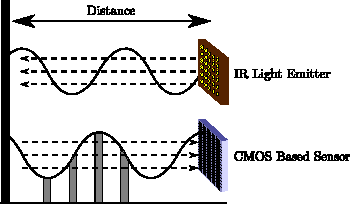
\includegraphics[width=0.5\linewidth]{Bilder/ToF_Principle.pdf}
	\caption{Principle of Continuous-wave Time-of-Flight \cite{foix2011lock}}
	\label{fig:tof_reflection}
\end{figure} 

The time window for the CW measurement is the integration time. It is comparable to the exposure time of an ordinary image sensor. Figure \ref{fig:tof_reflection} illustrates a radiated and reflected square wave IR signal and four phase shifted time windows. $Q_1$ to $Q_4$ represent the amount of charges that are collected in every window. In contrast to the pulsed control, the ambient light can be canceled out by measuring it out of the phase to the IR Signal \cite{litime}.

\begin{figure} [!h]
	\centering
	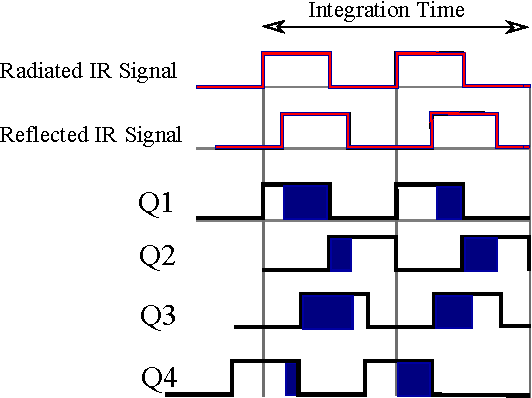
\includegraphics[width=0.5\linewidth]{Bilder/TOF_timing_diagram.pdf}
	\caption{Measuring windows of continuous-wave ToF}
	\label{fig:CW_principle}
\end{figure} 

\begin{equation}
\varphi = \arctan \frac{Q_3 - Q_4}{Q_1 - Q_2}
\end{equation}

\begin{equation}
d=\frac{c}{4\cdot \pi \cdot f}\cdot \varphi
\label{eq:ToF_distance}
\end{equation}
\medskip

The reflected amplitude A and the ambient light offset B are proportional to the depth measurement variance $\sigma^2$:

\begin{equation}
\sigma^2=\frac{c}{4 \cdot \sqrt{2} \cdot \pi \cdot f} \cdot \frac{\sqrt{A+B}}{c_d \cdot A}
\label{eq:variance}
\end{equation}\medskip

Equation \ref{eq:variance} shows that the variance can be reduced with a higher modulation frequency $f_{mod}$ and amplitudes A. The constant $c_d$ is a indicator, how well the ToF sensor separates and collects the photoelectrons. The amplitude can be increased with shorter distances to the scene or with a higher radiant intensity. One disadvantage of the CW measurement is that the phase warps around every $2\pi$. The ambiguity results in multiple possible distances. The intensity of the reflecting light helps to identify the true distance. This limits the range that can be observed. A reduction in the modulation frequency would increase the ambiguity distance but reduce the accuracy at the same time. With the maximum phase shift angle $\varphi = 2\cdot\pi$ and equation \ref{eq:ToF_distance}, the ambiguity distance can be calculated by the following equation:\\

\begin{equation}
d_{amb}=\frac{c}{2\cdot f_{mod}}
\end{equation}
\medskip

Ambient light in the same IR spectral region disturbs and results in noise. A monochromatic filter in front of the lens can reduce the incident light to the wavelength of the emitting diodes. Unfortunately, the sunlight emits in a broad bandwidth that cannot be filtered out completely.\\

 In comparison to the other range imaging techniques, ToF has the advantage of a small size, no moving parts, a high range and a very fast scanning speed. The only disadvantage is the low depth accuracy of $1~mm$. New senor developments could increase the resolution significantly down to $0.3~mm$ \cite{thierryoggietof}.

\subsection{Time-of-Flight Imaging Errors} \label{chap:range_errors}
Depth measurement with ToF cameras faces the appearance of both, systematic and non-systematic errors. Generally, systematic errors can be reduced by a calibration \cite{foix2011lock}. This section gives a rough overview of different errors sources and their reasons. 

\subsubsection{Systematic Errors}
\textbf{Range Distortion}\\
The IR light can not be generated in an ideal sinusodial or square waveform, as a consequence range distortion appears. Usually, the error plotted against the distance follows a sinusoidal shape that can be compensated by a calibration. \\

\textbf{Integration-Time-Related Error}\\
Scientific ToF cameras allow to adjust the integration time for the depth measurement. For the same scene, different values cause changes in the results. The precision versus different depths depends on the integration time.\\

\textbf{Build in Pixel-Related Errors}\\
Inaccuracies in the production of the image sensor causes error in the depth measurement. The diodes or capacitors differ in the responsibility and latency-related offset error. This type of errors are related to the position of the pixel on the sensor array. A Fixed Pattern Noise (FPN) table can be created to obtain the computed depth with a reference distance.\\

\textbf{Amplitude-Related Errors}\\
Depth accuracy is highly related to the amount of incident light. High reflected amplitudes result in a high accuracy. Low amplitudes appear more often at the border of the image as the emitted light power is lower. When the object is too close to the camera or the integration time has been chosen to high, saturation appears and the depth measurement will be invalid.\\

\textbf{Temperature-Related Errors}\\
Depth values suffer from the operation temperature of the sensor. After the activation of the camera it is heating up, until it reaches a stable temperature. In this phase, the depth error changes versus time. The camera should be turned on several minutes with activated illumination before the usage to achieve an precise measurement.

\subsubsection{Non-systematic Errors}

\textbf{Low Illuminated Regions}\\
Scenes that are not illuminated uniformly will suffer from regions with low illumination. This causes a high amount of noise and a reduction in the signal-to-noise ratio. The amplitude image can be used to filter out these kinds of pixels.\\

\textbf{Multiple Light Reflection Error}\\
The interference of different light reflection in a single pixel occurs depending on the shape of the scene. Surface edges and concavity reflect the wave in multiple ways. The light travels in successive paths before it reaches the sensor. Therefore, a depth measurement is corrupted. Flying pixels on sharp edges are one artifact that is observed in all ToF 3D scans. Light from the background interferes with the reflection on the edge in the foreground. This result is a noisy pixel that seams to jump in space and cannot be allocated to a connected surface.\\

\textbf{Light Scattering}\\
Reflections with high amplitudes from nearby objects can cause light scattering between the image sensor and its lens. This influences the measurement of other nearby pixels and results in noise. New sensor material with low reflectivity could make scattering negligible in the future.\\

\textbf{Motion Blur}\\
As with traditional cameras, the capture of dynamic scenes results in motion blur, depending on the integration time and the speed of the observed object. The error can be classified in two different types of artifacts: Lateral and axial blur.\\

\textbf{Flying Pixels}\\
False distance information can also occur due to the pixels relative large solid angle. Different distances inside a solid angle lead to superimposed reflected light reducing its amplitude and introducing a false phase shift. These pixels are commonly known as flying pixels, because they lie in-between the fore-and background. 


\newpage
\subsection{Acquisition of Digital Dynamic Data}

The discretization of an analog signal, like from a pixel, is done in the analog to digital converter (ADC). The signal value will be divided into single samples depending on the bit depth $n_{Bits}$ as shown in figure \ref{fig:nyquistthereom} with 3 Bits $\equiv 2^3$ steps. The sampling is controlled by a digital signal with the frequency $f_{sampling}$ that determines the conversion from the analog to the digital value. The Nyquist-Shannon theorem in equation \ref{eq:Nyquist-Shannon Theorem} proves, that the minimal possible sampling frequency $f_{sampling}$ must be double the maximum frequencies $f_{max}$ of the signal to preserve the spectrum. For the estimation of amplitude and slop a factor of two is not enough. A variety of samples per period is required, depending on the shape of the signal, to ensure a sample as near as possible to the peak of the deflection. High resolutions and sampling frequency mean less quantization errors. Therefore, differences between the digital and analog signal gets smaller. The averaging of multiple samples is a common way, used to reduce the noise and the data stream of the acquisition.

\begin{equation}
f_{sampling}\geq f_{nyquist} = f_{max} \cdot 2 
\label{eq:Nyquist-Shannon Theorem} 
\end{equation}

\begin{figure}[!h]
	\centering
	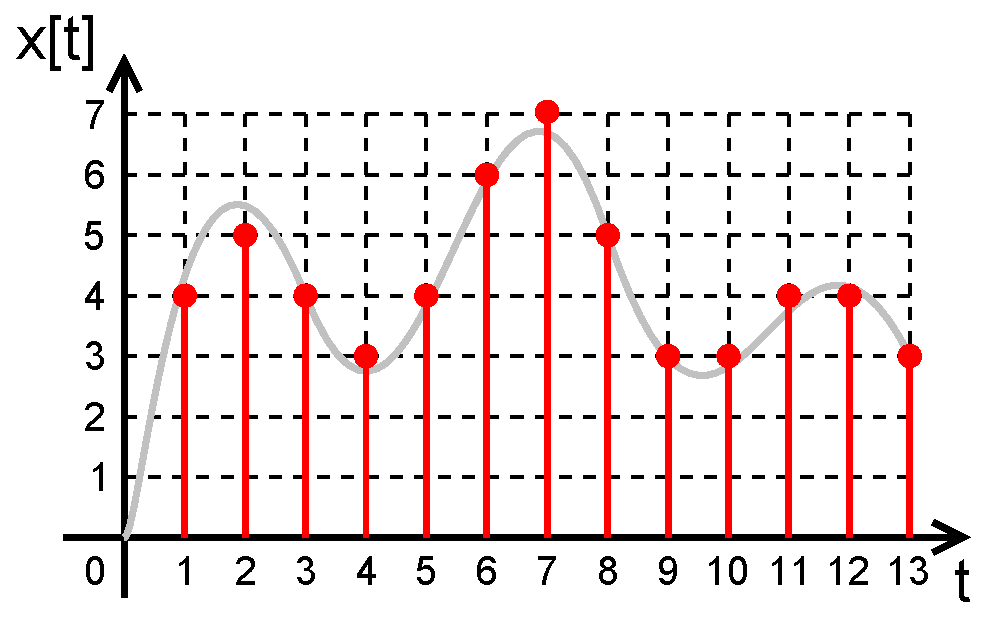
\includegraphics[width=0.4\textwidth]{Bilder/discret.pdf}
	\caption{Illustration of the analog to digital conversion \tiny wdwd wikipedia.org}
	\label{fig:nyquistthereom}
\end{figure}

Higher frequencies above $f_{max}$, resulting from noise or other sources, still have an undesirable impact on lower spectral components. These effects are called aliasing artifacts and lead to artificial frequency components. A low-pass filter applied on the analog signal with a cutoff frequency $f_{max}$ can reduce this phenomenon. Higher frequencies than $f_{max} = f_{sampling}~/~2$ will not arrive at the ADC input.\\

An aperture error results from the fact that the sample is obtained as a time average within a sampling region and not at an instant moment. The effects are corresponding to the motion blur of image sensors. Oversampling is the process of sampling with frequencies much higher than $f_{nyquist}$, leading to an improved resolution and less quantization noise. For an accurate measurement of the amplitude, a minimum sampling frequency of $f_{sampling} = f_{nyquist}\cdot 5$ is used in practice, to reduce influences like aperture errors or aliasing. The factor between the $f_{nyquist}$ and $f_{sampling}$ dimension is called Oversampling Factor N. The data stream of a ADC converter can be calculated by the sampling frequency $f_{sampling}$ and the digital resolution $n_{Bits}$ by the following equation:

\begin{equation}
\dot n = n_{Bits}\cdot f_{sampling} ~ [\frac{bit}{s}]
\label{eq:datastream} 
\end{equation}
 
\subsection{Evaluation of Dynamic Data}

\subsubsection{Time Domain}
The analysis of mathematical function with respect to time is called time domain. The time is represented in form of real numbers, for the case of continuous time or in discrete number resulting in a discrete time. An oscilloscope is a common tool for the investigation of real-world signals in the time domain. The graph describes how a value changes with time, whereas a frequency-domain graph describes how much of the signal amplitude lies within a given frequency band versus a range of frequencies. Certain terms are used for the description of the time domain. Figure \ref{fig:sinus} shows different properties of a sinus oscillation.  

\begin{figure}[!h]
	\centering
	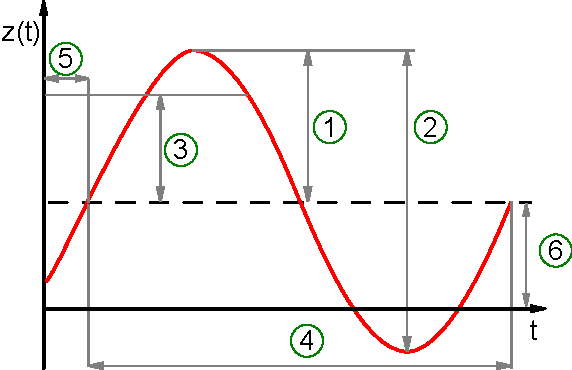
\includegraphics[width=0.4\textwidth]{Bilder/Sine_oscillation.pdf}
	\caption{Properties of sinus oscillation \tiny Saure wikipedia.org}
	\label{fig:sinus}
\end{figure}

\begin{enumerate}
\setlength\itemsep{0.001em} 
\item Peak amplitude $A_{p}$ - Maximum absolute value from zero to highest values
\item Peak-to-peak amplitude $A_{pp}=A_{p}\cdot 2$ - Change between highest value and lowest amplitude value
\item Root mean square amplitude $A_{rms}=A_{p}/\sqrt{2}$ - The square root of the mean versus time of the square in the vertical distance of the graph
\item Wave Periode $T=\frac{1}{f_{p}}=\frac{2*\pi}{\omega}$ - Time difference between one periodic oscillation
\item Phase Shift $\varphi$ - Time difference between the $t=0$ and the zero crossing of the oscillation or another reference time
\item Offset $Z_{DC} $ - Constant displacement from the origin to the equilibrium
\end{enumerate}	
	
An undamped sinus oscillation can be described in two mathematical forms: One is the common analytic sinus form as a function of time $t$. The value $Z_{DC}$ is a static offset in the coordinate system that superimposes the dynamic by a constant static value. In this case, the oscillation is not around the point of origin but around the equilibrium.

\begin{equation}
z(t)=A_{p}\cdot \sin(~2\cdot\pi \cdot f \cdot t + \varphi~) +Z_{DC}
\end{equation}  

The oscillation can also be represented with the help of the Euler equations and imaginary numbers. The imaginary part has no physical meaning, but it simplifies the processing of a dynamic function.
\begin{equation}
\bar{z}(t)=A\cdot e^{j(\omega\cdot t +\varphi)} + Z_{DC}
\end{equation}

The energy keeps constant at a free undamped sinus oscillation:

\begin{equation} \label{eq:Energy_oscillation}
E=\frac{1}{2}~m\omega^2 A^2
\end{equation}



\subsubsection{Frequency Domain} \label{chap:frequency_domain}
Every steady periodic function can be transformed into a sum of sinus oscillations, by a so called Fourier transformation. This allows the investigation and the comparison of dynamic signals. To do so, the data is transformed from the time domain $z(t)$ into the frequency domain $|Y(f)|$. The signals can now be investigated without a common time base. The frequency domain is represented by a spectrum that shows the individual amplitudes components versus the corresponding frequencies. This can be especially useful in the analysis of vibrations of structures. Undesired eigenmotions can be compared and analyzed. In figure \ref{fig:FFT_principle}, the waveform of equation \ref{eq:noise_fft} is illustrated, which is superimposed by some random noise.

\begin{equation} \label{eq:noise_fft}
z(t)= 0.7\cdot sin(2\cdot \pi\cdot 50~Hz \cdot t) + 1.4\cdot sin(2\cdot\pi\cdot 120~Hz \cdot t) + y_{noise}
\end{equation}

The two sinus wave forms and the noise are difficult to separate in the time domain. In the frequency domain, in contrast, noise and the original function can be distinguished. The two peaks indicate that the original function consists of two sinus functions with 50 Hz and 120 Hz. The noise floor lies underneath with multiple random peaks in the whole spectrum. The amplitudes from the original signal converge with the peaks in the frequency domain over a longer timespan and a higher $f_{sampling}$. More detailed information on this example can be found in the official Matlab documentation of the fft() function \cite{Matlab_FFT}.

\begin{figure}[!h]
	\subfigure[Time Domain]{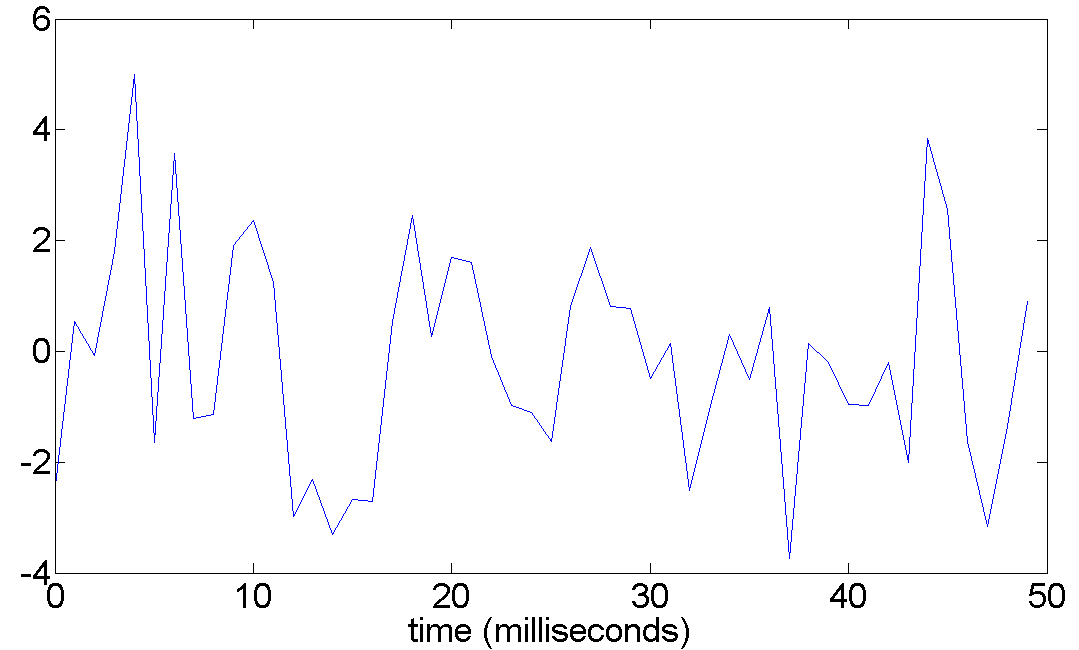
\includegraphics[width=0.5\textwidth]{Bilder/FFT_example_timedomain.png}}\hfill
	\subfigure[Frequency Domain]{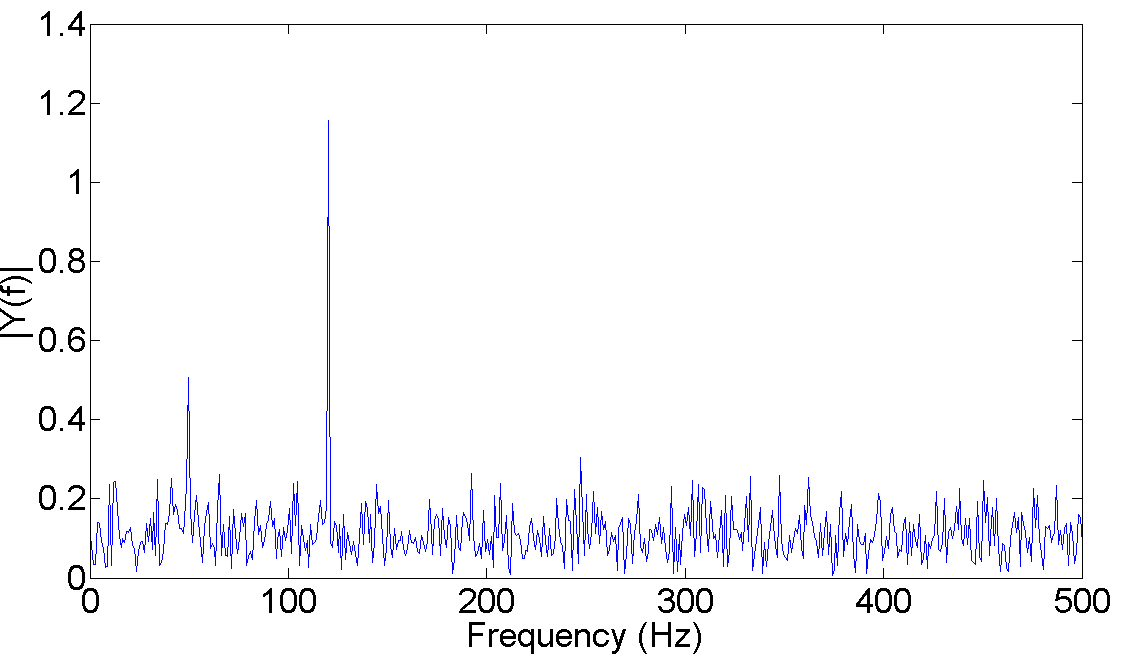
\includegraphics[width=0.52\textwidth]{Bilder/FFT_example_freqdomain.png}}
	\caption{Fast Fourier Transformation in Matlab}
	\centering
	\label{fig:FFT_principle} 
\end{figure}

The Fast Fourier transform (FFT) is a widely used algorithm to convert a digital signal from one domain into another. The input data must be in a discrete digital form with $2^n$ samples. In this way, the processing power is much lower compared to the original Discrete Fourier Transform (DFT). The signal is transformed into its complex components. The real parts of the frequencies represents half of the sinus function amplitude. $f_{sampling}$ of the computed signal must be known to calculate the right frequencies out of the raw data. The following code is take from the fft() example and plots the frequency domain out of the raw data array y with the number of elements L:

\begin{lstlisting} 
NFFT = 2^nextpow2(L); % Next power of 2 from length of y
Y = fft(y,NFFT)/L;
f = Fs/2*linspace(0,1,NFFT/2+1);
plot(f,2*abs(Y(1:NFFT/2+1)))
\end{lstlisting} 

NFFT contains the number of samples that are processed. Y is half of the amplitudes while f provides the corresponding frequency array that goes from zero to $f_{nyquist}$. These data are plotted against each other. The single-sides amplitude is two times the real part of the complex representation of the amplitude components from Y.\\
 
The original digital signal can be reproduced from the frequency domain into the time domain without any loss through the inverse fast Fourier transform. This is useful for the filtering of data. Undesired frequency components can be identified and removed from the data.
When the FFT of a non-periodic signal is computed, the resulting spectrum suffers from leakage. This can occur when only parts of a period are measured at the start or the end of the acquisition. The variance of the spectrum increases. Different FFT windows are used to reduce the influence of signal at the beginning and ending, like the hammington window \cite{proakis2001digital}. When measuring a self-windowing signal, like an impulse, a shock response, a sine burst or a noise burst a window should not be used. Such signals are used in modal analysis. Applying a window function would just deteriorate the signal-to-noise ratio.\\

The Short-time Fourier Transform (STFT) is used to determine the sinusoidal frequency and phase content of local sections of a signal as it changes versus time. Therefore variation versus time can be analyzed better than with the FFT of the complete signal. The Matlab function spectrogram() delivers a way to create a STFT out of a signal. The trend of amplitude and frequency is plotted versus time in intervals that are represented by NFFT as a number of samples for a separated Fourier Transform. The overlapping factor describes the range between two windows that is analyzed by both. The following source code represents an example for the creation of a spectrogram in Matlab:

\begin{lstlisting} 
 Fs = 30; %Samplingrate
 amp=2;%peak-Wert
 zeitmax=5;
 zeit=linspace(0,zeitmax,zeitmax*Fs);
 daten=amp*sin(2*pi*zeit*frequenz)
 nfft = 32;%Blockgroesse 2er-Potenz
 window = hanning(nfft);
 % z.B. 80 fuer 80% overlap
 Prozent_overlap = 5;
 overlap = round(nfft/100)*Prozent_overlap;
 [B,F,T] = spectrogram(daten,window,overlap,nfft,Fs)
 figure
 imagesc(T,F,abs(B));
 colormap(jet);
 colorbar
 axis xy
 ylim([0 30])
\end{lstlisting} 
 

\newpage
